% Options for packages loaded elsewhere
% Options for packages loaded elsewhere
\PassOptionsToPackage{unicode}{hyperref}
\PassOptionsToPackage{hyphens}{url}
\PassOptionsToPackage{dvipsnames,svgnames,x11names}{xcolor}
%
\documentclass[
  13pt,
]{article}
\usepackage{xcolor}
\usepackage[margin=2cm]{geometry}
\usepackage{amsmath,amssymb}
\setcounter{secnumdepth}{5}
\usepackage{iftex}
\ifPDFTeX
  \usepackage[T1]{fontenc}
  \usepackage[utf8]{inputenc}
  \usepackage{textcomp} % provide euro and other symbols
\else % if luatex or xetex
  \usepackage{unicode-math} % this also loads fontspec
  \defaultfontfeatures{Scale=MatchLowercase}
  \defaultfontfeatures[\rmfamily]{Ligatures=TeX,Scale=1}
\fi
\usepackage{lmodern}
\ifPDFTeX\else
  % xetex/luatex font selection
  \setmainfont[]{Times New Roman}
\fi
% Use upquote if available, for straight quotes in verbatim environments
\IfFileExists{upquote.sty}{\usepackage{upquote}}{}
\IfFileExists{microtype.sty}{% use microtype if available
  \usepackage[]{microtype}
  \UseMicrotypeSet[protrusion]{basicmath} % disable protrusion for tt fonts
}{}
\usepackage{setspace}
\makeatletter
\@ifundefined{KOMAClassName}{% if non-KOMA class
  \IfFileExists{parskip.sty}{%
    \usepackage{parskip}
  }{% else
    \setlength{\parindent}{0pt}
    \setlength{\parskip}{6pt plus 2pt minus 1pt}}
}{% if KOMA class
  \KOMAoptions{parskip=half}}
\makeatother
% Make \paragraph and \subparagraph free-standing
\makeatletter
\ifx\paragraph\undefined\else
  \let\oldparagraph\paragraph
  \renewcommand{\paragraph}{
    \@ifstar
      \xxxParagraphStar
      \xxxParagraphNoStar
  }
  \newcommand{\xxxParagraphStar}[1]{\oldparagraph*{#1}\mbox{}}
  \newcommand{\xxxParagraphNoStar}[1]{\oldparagraph{#1}\mbox{}}
\fi
\ifx\subparagraph\undefined\else
  \let\oldsubparagraph\subparagraph
  \renewcommand{\subparagraph}{
    \@ifstar
      \xxxSubParagraphStar
      \xxxSubParagraphNoStar
  }
  \newcommand{\xxxSubParagraphStar}[1]{\oldsubparagraph*{#1}\mbox{}}
  \newcommand{\xxxSubParagraphNoStar}[1]{\oldsubparagraph{#1}\mbox{}}
\fi
\makeatother


\usepackage{longtable,booktabs,array}
\usepackage{calc} % for calculating minipage widths
% Correct order of tables after \paragraph or \subparagraph
\usepackage{etoolbox}
\makeatletter
\patchcmd\longtable{\par}{\if@noskipsec\mbox{}\fi\par}{}{}
\makeatother
% Allow footnotes in longtable head/foot
\IfFileExists{footnotehyper.sty}{\usepackage{footnotehyper}}{\usepackage{footnote}}
\makesavenoteenv{longtable}
\usepackage{graphicx}
\makeatletter
\newsavebox\pandoc@box
\newcommand*\pandocbounded[1]{% scales image to fit in text height/width
  \sbox\pandoc@box{#1}%
  \Gscale@div\@tempa{\textheight}{\dimexpr\ht\pandoc@box+\dp\pandoc@box\relax}%
  \Gscale@div\@tempb{\linewidth}{\wd\pandoc@box}%
  \ifdim\@tempb\p@<\@tempa\p@\let\@tempa\@tempb\fi% select the smaller of both
  \ifdim\@tempa\p@<\p@\scalebox{\@tempa}{\usebox\pandoc@box}%
  \else\usebox{\pandoc@box}%
  \fi%
}
% Set default figure placement to htbp
\def\fps@figure{htbp}
\makeatother


% definitions for citeproc citations
\NewDocumentCommand\citeproctext{}{}
\NewDocumentCommand\citeproc{mm}{%
  \begingroup\def\citeproctext{#2}\cite{#1}\endgroup}
\makeatletter
 % allow citations to break across lines
 \let\@cite@ofmt\@firstofone
 % avoid brackets around text for \cite:
 \def\@biblabel#1{}
 \def\@cite#1#2{{#1\if@tempswa , #2\fi}}
\makeatother
\newlength{\cslhangindent}
\setlength{\cslhangindent}{1.5em}
\newlength{\csllabelwidth}
\setlength{\csllabelwidth}{3em}
\newenvironment{CSLReferences}[2] % #1 hanging-indent, #2 entry-spacing
 {\begin{list}{}{%
  \setlength{\itemindent}{0pt}
  \setlength{\leftmargin}{0pt}
  \setlength{\parsep}{0pt}
  % turn on hanging indent if param 1 is 1
  \ifodd #1
   \setlength{\leftmargin}{\cslhangindent}
   \setlength{\itemindent}{-1\cslhangindent}
  \fi
  % set entry spacing
  \setlength{\itemsep}{#2\baselineskip}}}
 {\end{list}}
\usepackage{calc}
\newcommand{\CSLBlock}[1]{\hfill\break\parbox[t]{\linewidth}{\strut\ignorespaces#1\strut}}
\newcommand{\CSLLeftMargin}[1]{\parbox[t]{\csllabelwidth}{\strut#1\strut}}
\newcommand{\CSLRightInline}[1]{\parbox[t]{\linewidth - \csllabelwidth}{\strut#1\strut}}
\newcommand{\CSLIndent}[1]{\hspace{\cslhangindent}#1}



\setlength{\emergencystretch}{3em} % prevent overfull lines

\providecommand{\tightlist}{%
  \setlength{\itemsep}{0pt}\setlength{\parskip}{0pt}}



 


\usepackage[noblocks]{authblk}
% packages needed by kableExtra tables (not recorded when chunks are cached)
\usepackage{multirow}
\usepackage{colortbl}
\renewcommand*{\Authsep}{, }
\renewcommand*{\Authand}{, }
\renewcommand*{\Authands}{, }
\renewcommand\Affilfont{\small}
\makeatletter
\@ifpackageloaded{caption}{}{\usepackage{caption}}
\AtBeginDocument{%
\ifdefined\contentsname
  \renewcommand*\contentsname{Table of contents}
\else
  \newcommand\contentsname{Table of contents}
\fi
\ifdefined\listfigurename
  \renewcommand*\listfigurename{List of Figures}
\else
  \newcommand\listfigurename{List of Figures}
\fi
\ifdefined\listtablename
  \renewcommand*\listtablename{List of Tables}
\else
  \newcommand\listtablename{List of Tables}
\fi
\ifdefined\figurename
  \renewcommand*\figurename{Figure}
\else
  \newcommand\figurename{Figure}
\fi
\ifdefined\tablename
  \renewcommand*\tablename{Table}
\else
  \newcommand\tablename{Table}
\fi
}
\@ifpackageloaded{float}{}{\usepackage{float}}
\floatstyle{ruled}
\@ifundefined{c@chapter}{\newfloat{codelisting}{h}{lop}}{\newfloat{codelisting}{h}{lop}[chapter]}
\floatname{codelisting}{Listing}
\newcommand*\listoflistings{\listof{codelisting}{List of Listings}}
\makeatother
\makeatletter
\makeatother
\makeatletter
\@ifpackageloaded{caption}{}{\usepackage{caption}}
\@ifpackageloaded{subcaption}{}{\usepackage{subcaption}}
\makeatother
\usepackage{bookmark}
\IfFileExists{xurl.sty}{\usepackage{xurl}}{} % add URL line breaks if available
\urlstyle{same}
\hypersetup{
  pdftitle={Do meritocratic beliefs undermine the acceptance of privilege at school-age? Evidence from a panel survey across students cohorts},
  pdfauthor={Juan Carlos Castillo; Tomás Urzúa; Andreas Laffert; René Canales; Kevin Carrasco},
  colorlinks=true,
  linkcolor={blue},
  filecolor={Maroon},
  citecolor={Blue},
  urlcolor={Blue},
  pdfcreator={LaTeX via pandoc}}


\title{Do meritocratic beliefs undermine the acceptance of privilege at
school-age? Evidence from a panel survey across students cohorts}


  \author{Juan Carlos Castillo}
            \affil{%
                  Department of Sociology, University of Chile
              }
        \author{Tomás Urzúa}
            \affil{%
                  Department of Sociology, University of Chile
              }
        \author{Andreas Laffert}
            \affil{%
                  Institute of Sociology, Pontifical Catholic University
                  of Chile
              }
        \author{René Canales}
            \affil{%
                  Institute of Sociology, Pontifical Catholic University
                  of Chile
              }
        \author{Kevin Carrasco}
            \affil{%
                  Department of Sociology, University of Chile
              }
      
\date{}
\begin{document}
\maketitle
\begin{abstract}
Schools are key spaces of meritocratic socialization, actively shaping
students' understanding of whether success is earned or inherited. Such
beliefs are central to students' sense of fairness, as they inform how
they interpret their own and others' outcomes, and whether they perceive
them as legitimate. Yet, there is still little knowledge about how
students conceive meritocracy and the way in which such conceptions
challenge the role of privilege in society. This study analyzes to what
extent perceptions and preferences about meritocracy and privilege
constitute distinct and related dimensions of students' beliefs, and how
they change over time and across school stages. Using a novel instrument
previously applied in adult population, we surveyed Chilean students in
6th and 9th grade (Wave 1: N = 846) and then in 7th and 10th grade (Wave
2: N = 662). Results support a multidimensional organization of
meritocratic and privilege beliefs, showing that endorsement to
meritocratic criteria can coexist with the acceptance of privilege
rather than displacing it. Besides, older students apply a more critical
frame when judging whether effort is rewarded in society. Taking into
account previous evidence in adult populations, these findings suggest
that youth meritocratic and privilege beliefs are shaped at early stages
of socialization, but they are also subject to change in a critical
direction as students mature.

\textbf{Keywords}: Meritocracy · Schools · Measurement invariance ·
Socialization · Chile
\end{abstract}


\setstretch{1.5}
\section{Introduction}\label{introduction}

The way in which children and youths come to understand who succeeds in
society and why is a relevant aspect of the socialization process
(\citeproc{ref-mijs_unfulfillable_2016}{Mijs, 2016};
\citeproc{ref-resh_sense_2014}{Resh \& Sabbagh, 2014}). Schools are
important actors in this regard, as they use grading, tracking, and
selection to apply meritocratic criteria based primarily on individual
talent and effort (\citeproc{ref-darnon_where_2018}{Darnon, Wiederkehr,
et al., 2018}; \citeproc{ref-traini_stratification_2022}{Traini, 2022}).
This early exposure to meritocratic principles in the ``impressionable
years'' (Krosnick \& Alwin (\citeproc{ref-krosnick_aging_1989}{1989}))
is consequential, as it shapes students' understanding of fairness and
incorporates notions of social mobility and social hierarchies. At the
same time, schools are environments where students encounter evidence
that outcomes are shaped by factors other than meritocratic ones, such
as family background, social connections, and structural advantages
(\citeproc{ref-bourdieu_reproduction_1990}{Bourdieu \& Passeron, 1990};
\citeproc{ref-goudeau_hidden_2017a}{Goudeau \& Croizet, 2017};
\citeproc{ref-tang_meritocratic_2025}{Tang et al., 2025}). These
background attributes can be considered privileges due to heritage-based
advantages over which people have no control, unlike effort. The
potential tension between meritocratic ideals and the weight of
privilege factors is a complex issue for students to navigate and is
central to their understanding of fairness and inequality. Yet, few
studies have explored how students conceive meritocracy and to what
extent such conceptions challenge the role of privilege in society.

Although meritocracy is often treated as a single dimension, mostly
related to individual effort, the literature growingly suggests that it
is a multidimensional construct. On the one hand, this refers to the
distinction between perceptions of how meritocracy operates in society
(``what is'') and preferences about how it should operate (``what ought
to be'') (\citeproc{ref-castillo_multidimensional_2023}{Castillo et al.,
2023}; \citeproc{ref-duru-bellat_whos_2012}{Duru-Bellat \& Tenret,
2012}). On the other hand, meritocratic beliefs can be distinguished
from privilege-based beliefs, which emphasize the role of family wealth
and social connections in shaping rewards in society
(\citeproc{ref-liu_does_2025}{C. Liu \& Wang, 2025};
\citeproc{ref-tang_meritocratic_2025}{Tang et al., 2025}). Such beliefs
also encompass perceptions of how society functions and preferences
about people's normative inclinations. In this sense, a multidimensional
approach incorporates perceptions and preferences about both
meritocratic and privilege-based explanations of social outcomes,
allowing for a more comprehensive understanding of how individuals
interpret social inequalities and fairness.

Previous research has shown that privilege and meritocratic beliefs
represent different and not necessarily opposite dimensions, therefore
they can coexist in people's minds
(\citeproc{ref-fan_disillusionment_2026}{Fan et al., 2026};
\citeproc{ref-liu_does_2025}{C. Liu \& Wang, 2025};
\citeproc{ref-tang_meritocratic_2025}{Tang et al., 2025}). This means,
for instance, that someone could believe that society rewards talent and
effort while also acknowledging that family wealth and social
connections play (or should play) a role in shaping outcomes. This
coexistence of beliefs has important implications for how individuals
understand social mobility, fairness, and inequality, as well as for how
they evaluate policies aimed at promoting equal opportunities. However,
attempts to study these beliefs have been limited by the lack of
instruments that capture their multidimensionality and by the absence of
longitudinal studies that examine how these beliefs evolve over time. In
the present study, we aim to contribute to the field of meritocracy
research by applying a multidimensional model to measure meritocratic
and privilege beliefs in a sample of Chilean students and by examining
the stability and measurement equivalence of these beliefs across school
stages and over time. Our main argument is that it is possible to
identify and distinguish meritocratic and privilege beliefs even at an
early school age, and that these beliefs have a structure similar to
that found in a previous study that applied the meritocracy framework in
the adult population
(\citeproc{ref-castillo_multidimensional_2023}{Castillo et al., 2023}).
Furthermore, we argue that these beliefs are not static, but rather
evolve over time as students gain more experience and exposure to
different social contexts.

This study draws on a two-wave panel dataset of Chilean students in 6th
and 9th grade (in wave 1). Studying meritocracy and privilege in the
context of Chilean schools provides a unique opportunity to explore how
students navigate the tension between meritocratic ideals and the
reality of social inequality. Chile's educational system combines high
stratification, market-based competition, and explicit meritocratic
discourse in school culture
(\citeproc{ref-castillo_socialization_2024}{Castillo et al., 2024};
\citeproc{ref-valenzuela_socioeconomic_2013}{Valenzuela et al., 2013}),
alongside persistent socioeconomic inequality and a deep marketization
of social welfare (\citeproc{ref-ferre_welfare_2023}{Ferre, 2023}),
features shared by many Latin American countries and increasingly
present in European and East Asian systems
(\citeproc{ref-busemeyer_skills_2014}{Busemeyer, 2014};
\citeproc{ref-gingrich_making_2011}{Gingrich, 2011}). This makes Chile a
productive case for studying how students internalize, question, or
reconcile meritocratic ideals with the reality of privilege, while the
dimensional structure and longitudinal patterns identified here are
likely to travel to other highly stratified educational contexts.

The research questions guiding this study are as follows:

\begin{enumerate}
\def\labelenumi{(\arabic{enumi})}
\item
  Do school-aged students distinguish between meritocratic and
  privilege-based principles, as well as between perceptions (``what
  is'') and preferences (``what should be'')?
\item
  Are the perceptions of privilege detrimental for the endorsement of
  meritocratic beliefs, or do they coexist in students' minds?
\item
  Are these dimensions stable over time and across school stages?
\end{enumerate}

In the following sections, we review the theoretical background on
meritocratic beliefs in school settings, present the methodology and
results, and discuss the implications of our findings for understanding
how meritocratic and privilege beliefs evolve during adolescence.

\section{Theoretical and empirical
background}\label{theoretical-and-empirical-background}

\subsection{The socialization of meritocracy at
school}\label{the-socialization-of-meritocracy-at-school}

Meritocracy refers to a distributive system in which individual merit,
typically defined as effort and personal ability, is treated as the
primary criterion for allocating resources and rewards, rather than
social origins or inherited privilege
(\citeproc{ref-bell_equality_1972}{Bell, 1972};
\citeproc{ref-young_rise_1958}{Young, 1958}). While Young
(\citeproc{ref-young_rise_1958}{1958}) coined the term as a dystopian
critique, it has since been re-appropriated as a positive ideal of
fairness in liberal and market-oriented societies
(\citeproc{ref-mijs_paradox_2021}{Mijs, 2021};
\citeproc{ref-vandewerfhorst_meritocracy_2024}{Van De Werfhorst, 2024}).
From a sociological standpoint, meritocracy operates both as a cognitive
judgment about how inequality works and as a moral lens through which
people evaluate whether unequal outcomes are deserved
(\citeproc{ref-castillo_meritocracia_2019}{Castillo et al., 2019};
\citeproc{ref-heuer_legitimizing_2020}{Heuer et al., 2020}). Precisely
because it frames outcomes as earned, meritocratic ideals have been
largely criticized as they could lead to reinforce inequality:
``winners'' are encouraged to see their position as deserved, while
``losers'' are pushed toward self-blame rather than structural critique
(\citeproc{ref-garcia-sierra_dark_2023}{García-Sierra, 2023};
\citeproc{ref-sandel_tyranny_2020}{Sandel, 2020}). In this line,
research in adult populations has documented systematic associations
between meritocratic beliefs and the justification of social
inequalities (\citeproc{ref-castillo_perceptions_2025}{Castillo et al.,
2025}; \citeproc{ref-liu_does_2025}{C. Liu \& Wang, 2025};
\citeproc{ref-mijs_paradox_2019}{Mijs, 2019};
\citeproc{ref-tejero-peregrina_perceived_2025}{Tejero-Peregrina et al.,
2025}). Despite the centrality of meritocratic beliefs for the
understanding of the social order, the question of how and when they
develop, and whether such beliefs are possible to identify in early
socialization stages has received few attention.

Schools are key institutions when it comes to the socialization of
meritocracy. On the one hand, they advance meritocratic ideals through
narratives of effort, achievement, self-improvement, and education as a
legitimate route to rewards and social mobility
(\citeproc{ref-batruch_belief_2022}{Batruch et al., 2022};
\citeproc{ref-chauvin_school_2026}{Chauvin et al., 2026};
\citeproc{ref-darnon_where_2018}{Darnon, Wiederkehr, et al., 2018};
\citeproc{ref-wiederkehr_belief_2015}{Wiederkehr et al., 2015}). On the
other hand, they embed these ideals in routine practices of grading,
tracking, selection, awards, and credentialing, which operate as
institutional markers of worth that make merit visible and consequential
in ways that are immediate and socially meaningful
(\citeproc{ref-resh_sense_2014}{Resh \& Sabbagh, 2014};
\citeproc{ref-traini_stratification_2022}{Traini, 2022}). This dual
character, at once cultural promotion and institutional enactment, is
what makes schools a particularly important arena for understanding how
meritocratic beliefs are formed and contested.

Along meritocratic socialization, schools are settings where
privilege-based advantages, including family resources, cultural
capital, peer environments, and unequal school quality, are also visible
and consequential (\citeproc{ref-batruch_belief_2022}{Batruch et al.,
2022}; \citeproc{ref-goudeau_hidden_2017a}{Goudeau \& Croizet, 2017};
\citeproc{ref-khan_saying_2013}{Khan \& Jerolmack, 2013}). This duality
can give rise to ambivalent or internally differentiated orientations.
Students may endorse meritocracy as a normative ideal while
simultaneously recognizing structural constraints, reflecting what the
literature describes as dual consciousness
(\citeproc{ref-liu_does_2025}{C. Liu \& Wang, 2025};
\citeproc{ref-tang_meritocratic_2025}{Tang et al., 2025}). This
coexistence is not fixed but can shift with educational experience: C.
Liu \& Wang (\citeproc{ref-liu_does_2025}{2025}) argue that education
can operate as either legitimation or enlightenment depending on the
broader inequality context, and longitudinal evidence suggests that
recognition of structural advantage tends to grow as students progress
through schooling (\citeproc{ref-tang_meritocratic_2025}{Tang et al.,
2025}). More broadly, meritocratic framing encourages students across
social backgrounds to interpret success and failure in individual terms,
reinforcing personal responsibility while limiting attention to
structural constraints (\citeproc{ref-darnon_where_2018}{Darnon,
Wiederkehr, et al., 2018}). As Lampert
(\citeproc{ref-lampert_meritocratic_2013}{2013}) argues, meritocratic
schooling can reward a minority while leading many others to internalize
failure as a personal deficiency, and even students from disadvantaged
backgrounds often adopt meritocratic narratives, suggesting that
prolonged exposure to school-based evaluation is a powerful mechanism
shaping beliefs about justice and inequality
(\citeproc{ref-henry_development_2006}{Henry \& Saul, 2006}).

The dynamics of meritocratic socialization are not static. Developmental
research suggests that by around age 10, children already articulate
judgments about social differences, typically emphasizing individual,
merit-based explanations while only beginning to incorporate
opportunity-based accounts (\citeproc{ref-imhoff_nociones_2025}{Imhoff
\& Brussino, 2025}; \citeproc{ref-sigelman_age_2013a}{Sigelman, 2013}).
As students move through the school system, however, cumulative exposure
to grading, tracking, peer comparison, and visible socioeconomic gaps
can make the limits of effort as a sufficient explanation for success
increasingly apparent. Tang et al.
(\citeproc{ref-tang_meritocratic_2025}{2025}) show that among Chinese
college students, those from lower socioeconomic backgrounds initially
report lower recognition of privilege-based advantages than their
higher-SES peers, but this gap narrows progressively across college
years as both groups converge toward stronger acknowledgment of
structural advantage. This trajectory suggests something important: it
is not simply that older students believe less in meritocracy, but that
sustained exposure to the educational system makes structural advantage
harder to ignore, generating what has been described as a ``reality
shock'' in which meritocratic discourse increasingly clashes with
experienced inequality (\citeproc{ref-allen_top_2016}{Allen, 2016}).
Adolescence is therefore a particularly consequential period for
studying these processes, precisely when abstract reasoning about
justice and fairness becomes more sophisticated and school-based sorting
mechanisms grow more salient
(\citeproc{ref-henry_development_2006}{Henry \& Saul, 2006};
\citeproc{ref-resh_sense_2014}{Resh \& Sabbagh, 2014}).

The consequences of these beliefs extend well beyond individual
attitudes. Students who perceive schools as highly meritocratic,
particularly believing that effort and talent are fairly rewarded, are
more likely to justify unequal access to social services, perceive class
inequalities as less unjust, express weaker support for redistribution,
and endorse stronger system-justifying beliefs
(\citeproc{ref-batruch_belief_2022}{Batruch et al., 2022};
\citeproc{ref-castillo_socialization_2024}{Castillo et al., 2024};
\citeproc{ref-wiederkehr_belief_2015}{Wiederkehr et al., 2015}). The
effects are not confined to students: among teachers, belief in school
meritocracy predicts preference for competitive over cooperative
classroom practices, while among parents it predicts lower demand for
policies aimed at reducing socioeconomic inequalities in achievement
(\citeproc{ref-darnon_competitive_2023}{Darnon et al., 2023}). These
patterns suggest that meritocratic beliefs are not merely attitudinal
outcomes of schooling but active inputs into the educational environment
itself, shaping classroom dynamics, institutional decisions, and the
broader normative climate in which students develop.

\subsection{Conceptualizing and measuring meritocratic and privilege
beliefs}\label{conceptualizing-and-measuring-meritocratic-and-privilege-beliefs}

The research agenda on meritocratic beliefs has faced challenges in
conceptualizing and measuring meritocracy. Some studies have relied on
narrow operationalizations that equate meritocracy with the social
valuation of effort (\citeproc{ref-mijs_paradox_2021}{Mijs, 2021};
\citeproc{ref-wiederkehr_belief_2015}{Wiederkehr et al., 2015}), often
reflecting simplified readings of Young's
(\citeproc{ref-young_rise_1958}{1958}) formulation (Merit = Effort +
Intelligence). For instance, the ``Preference for the Merit Principle
Scale'' (\citeproc{ref-davey_preference_1999}{Davey et al., 1999}) and
the ``Belief in School Meritocracy Scale''
(\citeproc{ref-batruch_belief_2022}{Batruch et al., 2022}) focus on the
perceived importance of effort and ability for success, while Wiederkehr
et al. (\citeproc{ref-wiederkehr_belief_2015}{2015}) measure the extent
to which respondents believe that hard work is rewarded. These
approaches, however, risk conflating meritocratic beliefs with general
attitudes toward effort or achievement, potentially overlooking the
broader structural and relational dimensions of meritocracy. Other
approaches treat meritocratic beliefs as interchangeable with broader
constructs such as system justification
(\citeproc{ref-day_movin_2017}{Day \& Fiske, 2017};
\citeproc{ref-jost_decade_2004a}{Jost et al., 2004}), beliefs about
social mobility (\citeproc{ref-deng_its_2025}{Deng \& Wang, 2025};
\citeproc{ref-mccoy_priming_2007}{McCoy \& Major, 2007}), or generalized
support for equal opportunity
(\citeproc{ref-batruch_belief_2022}{Batruch et al., 2022};
\citeproc{ref-darnon_where_2018}{Darnon, Wiederkehr, et al., 2018}). As
a result, attempts to measure meritocracy through questionnaire items
frequently collapse indicators that tap different dimensions, making it
difficult to assess what meritocracy actually means in practice.

A related, more specific limitation to study meritocracy concerns its
links with privilege-based factors such as family wealth, social
connections, and other structural advantages (Khan \& Jerolmack
(\citeproc{ref-khan_saying_2013}{2013})). As Castillo et al.
(\citeproc{ref-castillo_multidimensional_2023}{2023}) notes, much survey
research relies on item batteries that ask respondents to rate the
importance of effort, talent, family background, networks, or luck for
``getting ahead'', and then reduces these into a single score. This
becomes especially problematic when researchers construct continuum
measures in composite indicators, treating meritocratic and
privilege-based explanations as opposite ends of the same scale (e.g.,
by subtracting ``non-merit'' from ``merit,'' as in
\citeproc{ref-reynolds_perceptions_2014a}{Reynolds \& Xian, 2014}). Such
operationalizations embed a strong zero-sum assumption, namely that
endorsing merit necessarily entails rejecting structural or relational
advantages, thereby ruling out, by design, the empirical possibility
that both types of beliefs coexist. Recent debates, including the
exchange between Mijs (\citeproc{ref-mijs_visualizing_2026}{2026}) and
Wiesner \& Sachweh (\citeproc{ref-wiesner_effort_2026}{2026}),
underscore this point by arguing for measures that capture meritocratic
beliefs alongside privilege-based ones, rather than as a residual of the
relative importance assigned to structural factors. Complementary
empirical work has raised similar concerns: C. Liu \& Wang
(\citeproc{ref-liu_does_2025}{2025}) shows that meritocratic endorsement
may remain stable even as recognition of structural constraints
increases; Tang et al. (\citeproc{ref-tang_meritocratic_2025}{2025})
motivates dual consciousness but notes that operationalizations forcing
relative trade-offs risk obscuring it; Kwon \& Pandian
(\citeproc{ref-kwon_multidimensionality_2024}{2024}) identify three
attitudinal clusters in Europe, instrumental, idealized merit, and
ambivalent, showing that support for merit can coexist with recognition
of social connections in distinct configurations; and Zhu
(\citeproc{ref-zhu_meritocratic_2025}{2025}) argues directly that
meritocratic and structural explanations are not zero-sum but often
accumulate rather than replace one another. Unidimensional indices, and
especially subtraction scores, can therefore manufacture artificial
neutral positions and blur substantively distinct belief profiles that
carry different educational consequences.

In response to the identified limitations for the comprehensive
measurement of merit and privilege beliefs, Castillo et al.
(\citeproc{ref-castillo_multidimensional_2023}{2023}) proposed a
multidimensional framework that decomposes meritocratic beliefs along
two analytically independent axes: preferences versus perceptions, and
meritocratic versus privilege-based (originally called
``non-meritocratic'') allocation principles. Preferences capture
normative ideals about how rewards should be distributed (e.g., whether
effort and ability ought to determine life chances); perceptions capture
descriptive evaluations of how society actually works (e.g., whether
observed inequalities reflect merit-based processes)
(\citeproc{ref-janmaat_subjective_2013}{Janmaat, 2013}). Meritocratic
elements (effort, talent) and privilege-based elements (family wealth,
networks) are treated as distinct components rather than as opposites.
This yields four separate constructs, allowing belief combinations that
older measures tend to collapse, such as endorsing meritocracy as an
ideal while simultaneously recognizing the weight of family background
and connections. The proposal is deliberately minimalist, making it
well-suited for large-scale surveys with limited questionnaire space,
though this parsimony entails a trade-off: each factor is measured with
only two items, which can constrain reliability and content coverage.

Evidence from adult samples using confirmatory factor analysis supports
a four-factor structure (perceptions and preferences of both meritocracy
and privilege (\citeproc{ref-castillo_multidimensional_2023}{Castillo et
al., 2023}). Besides, it shows systematic associations among dimensions:
stronger perceived privilege tends to co-occur with stronger
meritocratic preferences
(\citeproc{ref-castillo_multidimensional_2023}{Castillo et al., 2023}),
a pattern that aligns with Zhu's
(\citeproc{ref-zhu_meritocratic_2025}{2025}) notion of dual
consciousness, here understood as the simultaneous endorsement of
meritocracy as a normative ideal alongside descriptive recognition that
rewards are shaped by structural advantage. Regarding school-based
research, these measurement challenges have received limited attention.
Chauvin et al. (\citeproc{ref-chauvin_school_2026}{2026}) propose a
multidimensional measure of school meritocracy that distinguishes
between equity and ability dimensions, but their scale applies only to
teachers and remains restricted to perceived meritocracy. Castillo et
al. (\citeproc{ref-castillo_socialization_2024}{2024}) apply the
four-factor framework to a sample of Chilean 10th graders and report
that students differentiate perceptions from preferences and
meritocratic from privilege-based principles; however, that study relies
on item-level descriptives and bivariate associations rather than a
formal factorial measurement model. Beyond this, to our knowledge no
study has examined whether these dimensions are stable across age
cohorts or over time, which limits understanding of how meritocratic
beliefs develop through schooling and whether observed differences
across stages reflect substantive change or measurement non-equivalence.

\subsection{This study}\label{this-study}

Building on the previous evidence, we state the following research
hypotheses:

\textbf{\(H_1\) (Dimensional differentiation)}: Students' meritocratic
and privilege beliefs can be represented and measured by four distinct
factors: perceived meritocracy, perceived privilege, meritocratic
preferences, and privilege acceptance.

\textbf{\(H_2\) (Beliefs compatibility)}: merit and privilege beliefs
are not mutually exclusive, but rather compatible orientations that can
coexist within the same individual.

\textbf{\(H_3\) (Equivalence)}: The four-factor model is equivalent
across the two waves of the panel survey and across two age cohorts (6th
and 9th grade in the first wave).

\section{Methods}\label{methods}

\subsection{Participants}\label{participants}

This study uses secondary data from the 2023 and 2024 waves of the Panel
Survey on Education and Meritocracy (EDUMER), which examines school-age
students' beliefs, attitudes, and behaviors regarding meritocracy,
inequality, and citizenship. The questionnaire was administered to
sixth-grade and first-year secondary students in nine schools in Chile's
Metropolitan and Valparaíso regions. Although the sample was
non-probabilistic and lacked quota controls, a minimum target of 900
students was set to ensure adequate statistical power. After data
processing and listwise deletion, the analytical sample included 846
students in Wave 1 (386 girls, 421 boys, 39 identifying as other;
\(M_{age}\) = 13.4, \(SD_{age}\) = 1.6) and 662 in Wave 2 (303 girls,
338 boys, 21 identifying as other; \(M_{age}\) = 14.4, \(SD_{age}\) =
1.6), yielding a retention rate of 78.3\% (attrition = 21.7\%). The main
sources of attrition were school transfers between academic years and
high absenteeism in several schools.

To distinguish students' academic level across waves for conditional and
multi-group invariance analyses, we created a cohort indicator capturing
whether the respondent belonged to the primary (sixth grade) or
secondary (first-year secondary) cohort at the time of each survey wave.
Descriptive statistics by cohort and wave are reported in
Table~\ref{tbl-cohort}.

\begin{table}[H]

\caption{\label{tbl-cohort}Descriptive statistics for cohort level}

\centering{

\centering\begingroup\fontsize{9.5}{11.5}\selectfont

\resizebox{\ifdim\width>\linewidth\linewidth\else\width\fi}{!}{
\begin{tabular}{>{\raggedright\arraybackslash}p{1.8cm}>{\raggedright\arraybackslash}p{2.2cm}>{\raggedleft\arraybackslash}p{1.6cm}>{\raggedleft\arraybackslash}p{1.6cm}>{\raggedleft\arraybackslash}p{1.6cm}>{\raggedleft\arraybackslash}p{1.9cm}>{\raggedleft\arraybackslash}p{1.9cm}>{\raggedleft\arraybackslash}p{1.9cm}}
\toprule
\multicolumn{3}{c}{ } & \multicolumn{2}{c}{Age} & \multicolumn{3}{c}{Gender} \\
\cmidrule(l{3pt}r{3pt}){4-5} \cmidrule(l{3pt}r{3pt}){6-8}
Wave & Cohort level & N & Mean & SD & Man & Women & Others\\
\midrule
 & Primary & 406 & 11.85 & 0.56 & 195 & 191 & 20\\
\cmidrule{2-8}
 & Secondary & 440 & 14.79 & 0.80 & 226 & 195 & 19\\
\cmidrule{2-8}
\multirow{-3}{1.8cm}{\raggedright\arraybackslash Wave 1} & Total & 846 & 13.38 & 1.63 & 421 & 386 & 39\\
\cmidrule{1-8}
 & Primary & 319 & 12.83 & 0.55 & 161 & 145 & 13\\
\cmidrule{2-8}
 & Secondary & 343 & 15.76 & 0.75 & 177 & 158 & 8\\
\cmidrule{2-8}
\multirow{-3}{1.8cm}{\raggedright\arraybackslash Wave 2} & Total & 662 & 14.35 & 1.61 & 338 & 303 & 21\\
\bottomrule
\end{tabular}}
\endgroup{}

}

\end{table}%

\subsection{Procedure}\label{procedure}

Data were collected by a professional research firm using a
Computer-Assisted Web Interviewing (CAWI) approach, based on online
questionnaires. All participants received informed consent, which was
reviewed and approved by a parent or legal guardian. To enable
longitudinal linkage while protecting confidentiality, the survey firm
generated anonymous unique identifiers for each student, and no directly
identifying information was included in the analytic files. Following
the principles of open science, the hypotheses were pre-registered on
the Open Science Framework (OSF) prior to data collection, and the
analytic code and data are publicly available on a public Github
repository .

\subsection{Measures}\label{measures}

\subsubsection{Perceptions and preferences of
meritocracy}\label{perceptions-and-preferences-of-meritocracy}

Meritocratic and privilege-based perceptions and preferences were
measured using the same items proposed in the original scale
(\citeproc{ref-castillo_multidimensional_2023}{Castillo et al., 2023}).
Each of the four dimensions of the scale is measured by two items. The
dimensions are:

\begin{itemize}
\item
  Meritocratic perceptions: the extent to which effort and ability are
  rewarded in Chile,
\item
  Privilege perceptions: the extent to which success is perceived as
  linked to connections and family wealth,
\item
  Meritocratic preferences: agreement with that those who work harder or
  are more talented should be better rewarded,
\item
  Privilege acceptance: agreement that it is acceptable for individuals
  with better connections or wealthy parents to achieve greater success
  (see Table~\ref{tbl-merit}).
\end{itemize}

Each item is rated on a four-point scale ranging from ``strongly
disagree'' (1) to ``strongly agree'' (4), therefore higher scores
indicate stronger endorsement of the corresponding perception or
preference.

\begin{table}[H]

\caption{\label{tbl-merit}Items for perceptions and preferences for
meritocracy scale}

\centering{

\centering\begingroup\fontsize{9.5}{11.5}\selectfont

\resizebox{\ifdim\width>\linewidth\linewidth\else\width\fi}{!}{
\begin{tabular}{>{\raggedright\arraybackslash}p{2cm}>{\raggedright\arraybackslash}p{2 cm}>{\raggedright\arraybackslash}p{6.5cm}>{\raggedright\arraybackslash}p{6.5cm}}
\toprule
Components & Dimensions & Item (English) & Item original (Spanish)\\
\midrule
 &  & In Chile people are rewarded for their efforts & En Chile las personas son recompensadas por sus esfuerzos\\
\cmidrule{3-4}
 & \multirow{-2}{2 cm}{\raggedright\arraybackslash Meritocratic} & In Chile people are rewarded for their intelligence and ability & En Chile las personas son recompensadas por su inteligencia y habilidad\\
\cmidrule{2-4}
 &  & In Chile those with wealthy parents do much better in life & En Chile a quienes tienen padres ricos les va mucho mejor en la vida\\
\cmidrule{3-4}
\multirow{-4}{2cm}[0.5\dimexpr\aboverulesep+\belowrulesep+\cmidrulewidth]{\raggedright\arraybackslash Perception} & \multirow{-2}{2 cm}{\raggedright\arraybackslash Privilege} & In Chile those with good contacts do much better in life & En Chile a quienes tienen buenos contactos les va mejor en la vida\\
\cmidrule{1-4}
 &  & Those who work harder should reap greater rewards than those who work less hard & Quienes más se esfuerzan deberían obtener mayores recompensas que quienes se esfuerzan menos\\
\cmidrule{3-4}
 & \multirow{-2}{2 cm}{\raggedright\arraybackslash Meritocratic} & Those with more talent should reap greater rewards than those with less talent & Quienes poseen más talento deberían obtener mayores recompensas que quienes poseen menos talento\\
\cmidrule{2-4}
 &  & It is good that those who have rich parents do better in life & Está bien que quienes tengan padres ricos les vaya mejor en la vida\\
\cmidrule{3-4}
\multirow{-4}{2cm}[0.5\dimexpr\aboverulesep+\belowrulesep+\cmidrulewidth]{\raggedright\arraybackslash Preference} & \multirow{-2}{2 cm}{\raggedright\arraybackslash Privilege} & It is good that those who have good contacts do better in life & Está bien que quienes tengan buenos contactos les vaya mejor en la vida\\
\bottomrule
\end{tabular}}
\endgroup{}

}

\end{table}%

\subsection{Analytical strategy}\label{analytical-strategy}

\subsubsection{Measurement model and
estimation}\label{measurement-model-and-estimation}

To address the multidimensional nature of meritocracy conceptual
framework, we estimated a Confirmatory Factor Analysis (CFA) based on a
measurement model with four latent factors. The estimation is performed
using Diagonally Weighted Least Squares with robust correction (WLSMV)
which is suitable for ordinal items.
(\citeproc{ref-kline_principles_2023}{Kline, 2023}). Model fit was
assessed following the guidelines of Brown
(\citeproc{ref-brown_confirmatory_2015}{2015}), using several indices:
the Comparative Fit Index (CFI) and the Tucker-Lewis Index (TLI), with
acceptable values above 0.95; the Root Mean Square Error of
Approximation (RMSEA), with values below 0.06 indicating good fit; and
the Chi-square statistic (acceptable fit indicated by \(p\)
\textgreater{} 0.05 and a Chi-square/df ratio \textless{} 3).

\subsubsection{Measurement equivalence across time and
groups}\label{measurement-equivalence-across-time-and-groups}

A key contribution of this study is its assessment of measurement
stability through factorial invariance testing
(\citeproc{ref-putnick_measurement_2016}{Putnick \& Bornstein, 2016}).
The objective of applying factorial invariance in this case is twofold:
first, as a robust test of the measurement model, and second, to ensure
that the latent constructs allow for valid comparisons across time and
groups. In this sense, the logic of factorial invariance is that the
same latent construct should be measured in the same way across time and
groups, so that any observed differences in the latent construct can be
attributed to true differences rather than measurement artifacts. In
this study, we tested for factorial invariance across two panel waves
(longitudinal invariance) and across school levels (comparing primary
vs.~secondary students cohorts). The logic of factorial invariance
testing is to compare a series of nested models with increasing
constraints, starting from a configural model (same factor structure
across time or groups) to more restrictive models that constrain factor
loadings, thresholds/intercepts, and residual variances .

We followed recent recommendations for ordered categorical indicators,
specifically the longitudinal approach of Y. Liu et al.
(\citeproc{ref-liu_testing_2017}{2017}) and the cross-group procedure as
suggested by Svetina et al.
(\citeproc{ref-svetina_multiplegroup_2020}{2020}). In addition to the
chi-square difference test, we assessed invariance using changes in
approximate fit indices. Following Chen
(\citeproc{ref-chen_sensitivity_2007}{2007}), we treated \(\Delta\)CFI
as the primary criterion and \(\Delta\)RMSEA as supplementary,
indicating noninvariance when \(\Delta\)CFI \(\geq\) −0.010 and
\(\Delta\)RMSEA \(\geq\) 0.015.

All analyses were performed using the \emph{lavaan} package in R version
4.5.2. The hypotheses of this research were
\href{https://osf.io/hjat2/}{pre-registered} on the Open Science
Framework (OSF).

\section{Results}\label{results}

This section is organized into three parts, each one referred to
corresponding three research questions and hypotheses. First, we present
descriptive statistics and visualizations of the survey items measuring
meritocratic perceptions and preferences, as well as perceived privilege
and its acceptance. Second, we report the results of the confirmatory
factor analysis (CFA) conducted to evaluate the proposed four-factor
structure of meritocratic perceptions, meritocratic preferences,
perceived privilege, and privilege acceptance. Based on in these results
we analyze the associations between the different dimensions of
meritocracy and privilege, which is at the core of our investigation.
Finally, we present the results of multigroup analyses to assess
measurement invariance across cohorts and waves.

\subsection{Descriptives}\label{descriptives}

Figure~\ref{fig-likerplot1} displays the response distributions for the
meritocracy and privilege items by each survey wave, distinguishing
perceptions from preferences. A clear and stable gap emerges between how
students perceive social rewards to operate and how they think they
should operate. In the perception items, agreement is consistently high
for contacts, parental wealth, and talent, whereas effort displays the
lowest perception. In the preference items, by contrast, effort is
overwhelmingly endorsed as the legitimate basis for rewards, exceeding
by far its perceived role in practice. Noticeably, in terms of
preferences, is the talent item the one showing the lower frequency,
being the use of contacts and family resources more preferred than this
meritocratic stance. Roughly, more that half of respondents in both
waves express an acceptance of the influence of rich parents and
contacts, revealing that such privilege criteria are not uniformly seen
as illegitimate way to get ahead.

\begin{figure}

\caption{\label{fig-likerplot1}Distribution of responses on the scale of
perceptions and preferences regarding meritocracy by wave}

\centering{

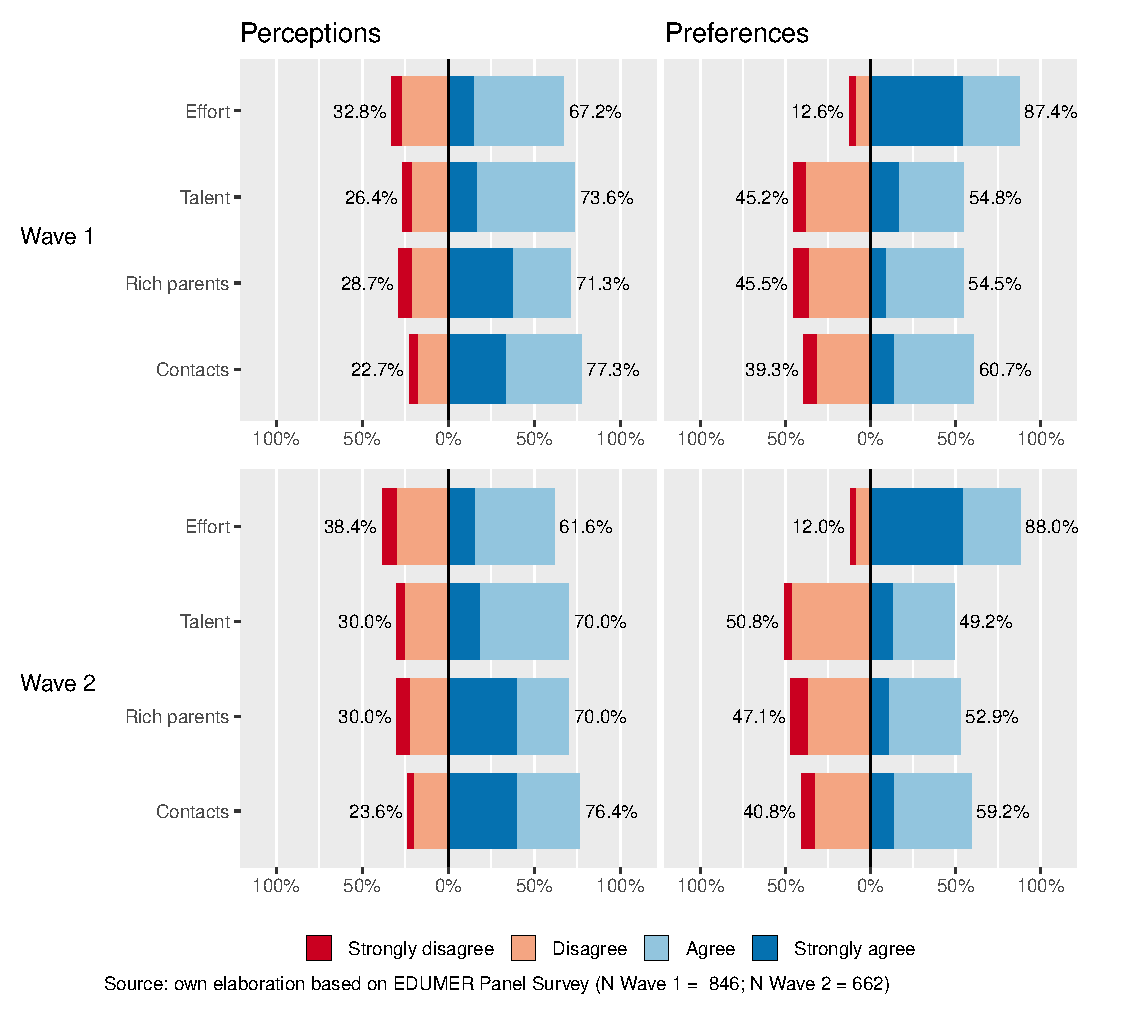
\includegraphics[width=1\linewidth,height=\textheight,keepaspectratio]{paper_files/figure-pdf/fig-likerplot1-1.pdf}

}

\end{figure}%

Regarding the primary and secondary education cohorts, some contrasts
emerge as seen in Figure~\ref{fig-likerplot2}. In terms of perception,
the meritocratic items (effort and talent) are the ones with the highest
agreement in the youngest cohort and the lowest in the oldest one. At
the same time, the privilege perceptual items (contacts and family
wealth) are the ones with the lowest agreement in the youngest cohort
and the highest in the oldest one. This pattern is consistent with
evidence on a ``disillusionment'' with meritocracy as students progress
through the educational system
(\citeproc{ref-fan_disillusionment_2026}{Fan et al., 2026};
\citeproc{ref-tang_meritocratic_2025}{Tang et al., 2025}). In terms of
preferences, the pattern is more stable across cohorts, with effort
being the most endorsed legitimate basis for reward, while talent,
family wealth, and especially contacts remain more ambivalent. As in the
previous descriprive analysis by wave, contacts are more often accepted
than rejected in both cohorts. Overall, the cohort comparison reveals a
widening gap between an effort-centered meritocratic ideal and the
perceived importance of privilege advantages in practice.

\begin{figure}

\caption{\label{fig-likerplot2}Distribution of responses on the scale of
perceptions and preferences regarding meritocracy by cohort}

\centering{

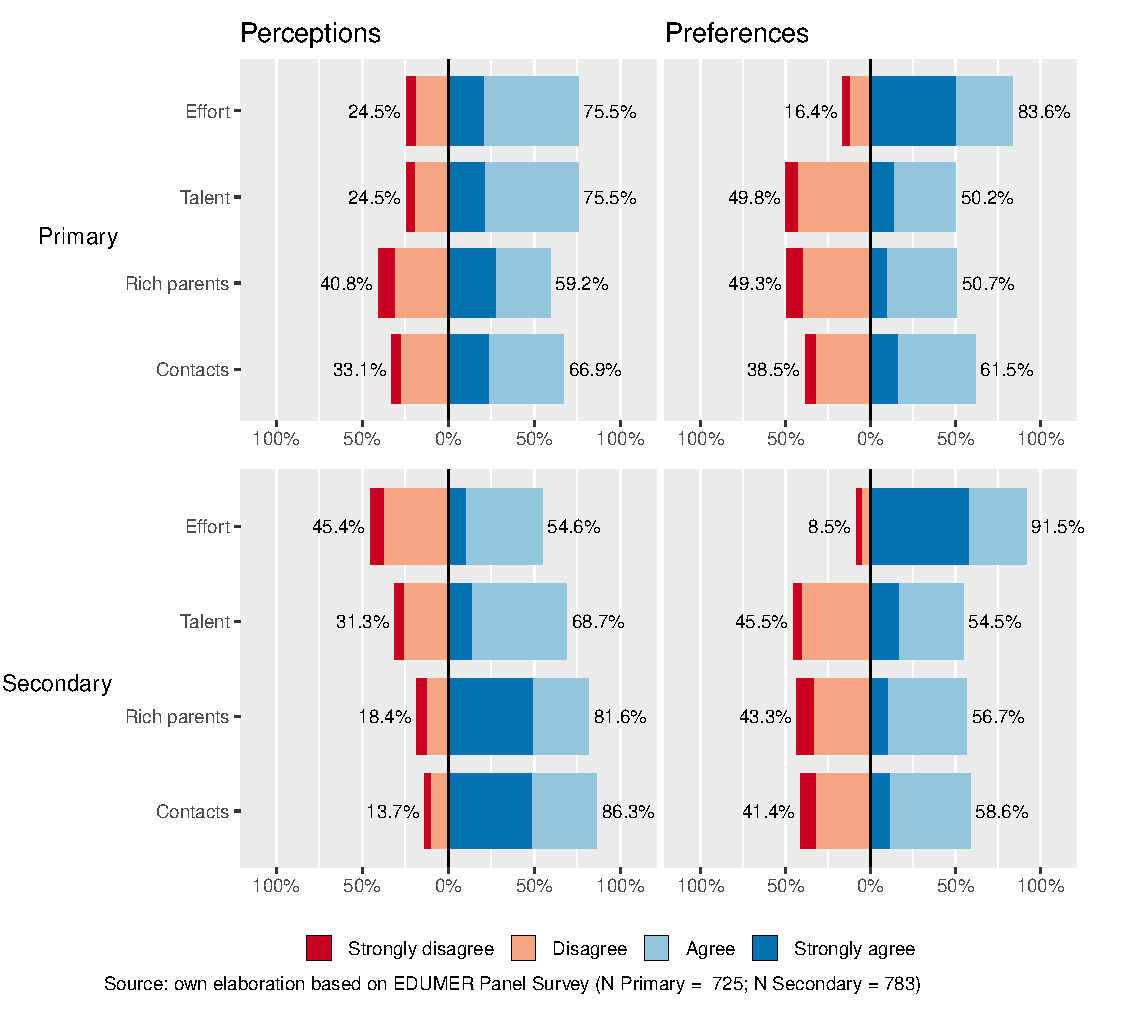
\includegraphics[width=1\linewidth,height=\textheight,keepaspectratio]{paper_files/figure-pdf/fig-likerplot2-1.pdf}

}

\end{figure}%

\subsection{Multidimensional measurement of meritocracy and
privilege}\label{multidimensional-measurement-of-meritocracy-and-privilege}

The eitgh items described in the previous section are conceptually
organized into four latent dimensions: meritocratic perceptions,
meritocratic preferences, perceived privilege, and privilege acceptance.
Previous research in adult population has shown that these dimensions
are empirically distinguishable and can be measured with a four-factor
structure (\citeproc{ref-castillo_multidimensional_2023}{Castillo et
al., 2023}). In this study, we extend this line of research to the
adolescent population, examining whether the same four-factor structure
holds in our sample of students from primary and secondary education
cohorts (\(H_1\)).

Figure~\ref{fig-general} presents a diagram of the general measurement
model. The hypothesized four latent dimensions are represented by
circles in the middle, each correspondig to two observed indicators
(rectangles) that are expected to load on the corresponding latent
factor. The arrows indicate the direction of the hypothesized
relationships, with factor loadings representing the strength of the
association between each indicator and its latent construct. The model
also allows for correlations among the four latent factors, reflecting
the potential interrelationships between meritocratic perceptions,
meritocratic preferences, perceived privilege, and privilege acceptance.
The model shows a reasonable --though not fully satisfactory-- fit to
the data (CFI = 0.97; TLI = 0.94; RMSEA = 0.07). Although the CFI falls
within commonly accepted ranges, the RMSEA and TLI remain below
conventional thresholds, indicating that fit is acceptable in some
respects but not uniformly strong across indices. As we will see later
on, part of the misfit relates to some differences across cohorts, which
are explored in the subsequent multigroup analyses.

\begin{figure}

\caption{\label{fig-general}Measurement model diagram (pooled sample)}

\centering{

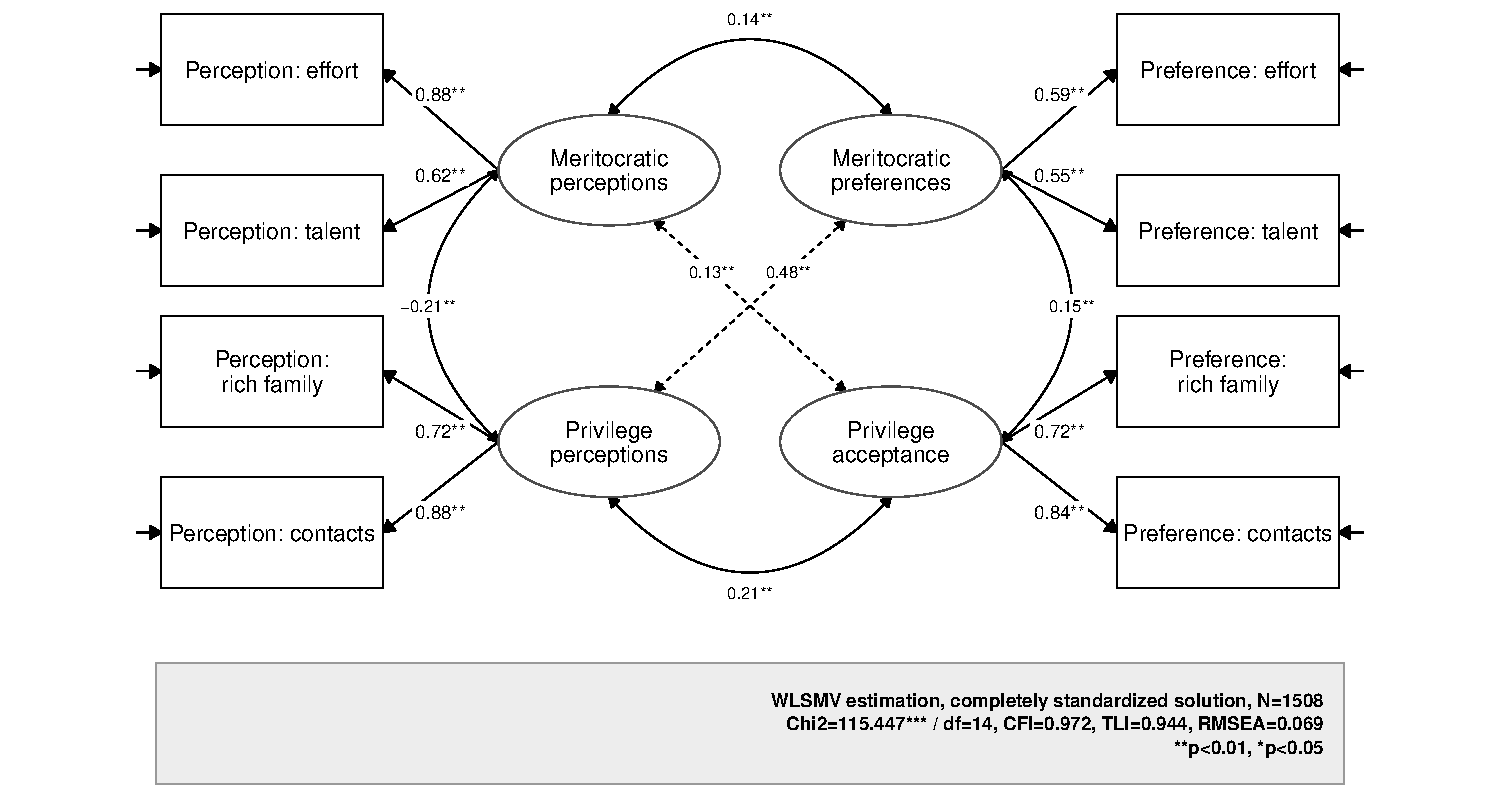
\includegraphics[width=1\linewidth,height=\textheight,keepaspectratio]{paper_files/figure-pdf/fig-general-1.pdf}

}

\end{figure}%

All standardized factor loadings are statistically significant and
generally moderate to strong, though their magnitude varies across
dimensions. For meritocratic perceptions, the effort item shows a
particularly strong loading (\(\beta\) = 0.88) and talent a moderately
strong loading (\(\beta\) = 0.62). Meritocratic preferences exhibit more
even, but somewhat weaker, loadings for effort (\(\beta\) = 0.59) and
talent (\(\beta\) = 0.55). For perceived privilege, both indicators load
strongly, especially contacts (\(\beta\) = 0.88), followed by coming
from a rich family (\(\beta\) = 0.72). Privilege acceptance also shows
strong and relatively balanced loadings, with contacts (\(\beta\) =
0.84) and rich family (\(\beta\) = 0.72), indicating that both
indicators are similarly representative of this latent dimension. In
general, the factor loadings suggest that the observed indicators are
reasonably good measures of their respective latent constructs, with
some variation in strength across dimensions.

The analysis of latent correlations gives us important insights into the
relationships among the four dimensions (\(H_2\)). As stated before,
allowing these for dimensions to correlate pertmit us to open the
black-box of meritocracy and privilege beliefs, which both in the common
sense as well as in the literature are often treated as the oposite
poles of a single continuum. The results show that the four dimensions
are indeed interrelated, but not perfectly aligned, indicating that
students' beliefs about meritocracy and privilege are complex and
multifaceted. To begin with, all the correlations but one are actually
positive. The only negative correlation is between meritocratic
perceptions and privilege perceptions, which is consistent with the idea
that perceiving society as more meritocratic is associated with a lower
recognition of the role of privilege (and vice versa). Some positive
associations also show a more intuitive pattern, such as the positive
correlation between meritocratic perceptions and meritocratic
preferences, suggesting that students who perceive society as more
meritocratic also tend to endorse meritocratic ideals. The strongest
association is between privilege perceptions and meritocratic
preferences, indicating that students who recognize the role of
privilege in society are also more likely to endorse meritocratic
ideals. However, other correlations suggest relationships that are less
straightforward, as for instance the positive correlation between
meritocratic preferences and privilege acceptance, which may indicate
that despite perceiving meritocracy, students may still accept the
legitimacy of privilege advantages. Something similar occurs with
positive association between meritocratic and privilege preferences,
which may suggest that students who endorse meritocratic ideals may also
recognize the legitimacy of privilege advantages. Although these last
correlations are modest in size, they highlight the complexity of
students' beliefs about meritocracy and privilege, suggesting that these
dimensions are not simply opposites but rather can coexist in students
minds without necessarily undermining one another.

\subsection{Stability of meritocracy and privilege
beliefs}\label{stability-of-meritocracy-and-privilege-beliefs}

This section objective is twofold. On the one hand, we aim at testing
the validity of the measurement model through an assessment of it
stability over time and cohorts. For this, we perform an assessment of
model equivalence or \emph{invariance}, which is a form of robustness
check that allows us to determine whether the latent constructs are
being measured in the same way across different groups or time points.
Such evidence is crucial for ensuring that any observed differences in
the latent constructs are not due to measurement artifacts but rather
reflect valid
differences(\citeproc{ref-putnick_measurement_2016}{Putnick \&
Bornstein, 2016}) . The test of the equivalence of parameters in a
confirmatory factor analysis follows a hierarchical approach, starting
with configural invariance (same factor structure across groups or time
points), then weak invariance (equal factor loadings), strong invariance
(equal intercepts), and finally strict invariance (equal residual
variances). Each level of invariance provides increasingly stringent
evidence that the measurement model is stable across groups or time
points. In this study, we first test for longitudinal invariance across
the two waves of data collection, and then we test for cohort invariance
between primary and secondary education students.

\subsubsection{Longitudinal invariance}\label{longitudinal-invariance}

Table~\ref{tbl-longinv} reports the results of the longitudinal
invariance tests. The logic of longitudinal invariance is to apply
senquential constraints to the model parameters across time, in order to
check to what extent the parameters are invariant across time. This is
basically takign the two measurement points as two comparing groups, but
in this case, the groups are the same individuals measured at two
different time points, which is incorporated in the model by correlating
the unique item variances. The table shows the fit indices for the
configural, weak (metric), strong (scalar), and strict invariance
models, along with the chi-square difference tests comparing each nested
model. Overall, the scale achieved the strongest level of invariance
(strict invariance) across the two waves. The strict model showed good
fit, \(\chi^2\)(84) = 130.17, CFI = 0.991, RMSEA = 0.031 (90\% CI:
0.020--0.040). Moreover, compared with the strong (scalar) model, the
deterioration in fit was negligible: \(\Delta \chi^2\)(4) = 1.635,
\(\Delta\)CFI = 0.000, and \(\Delta\)RMSEA = -0.002. These differences
fall well within commonly used cutoffs for invariance evaluation
(\citeproc{ref-chen_sensitivity_2007}{Chen, 2007}), indicating that
constraining residual variances in addition to loadings and
thresholds/intercepts is tenable. Substantively, this implies that the
item--factor relations are stable over time (metric invariance) and
that, for a given level of the latent trait, respondents are expected to
endorse the same response categories across waves (scalar invariance),
supporting the comparability of scores and latent parameters within
students over time.

\begin{table}[H]

\caption{\label{tbl-longinv}Longitudinal invariance results}

\centering{

\centering\begingroup\fontsize{9.5}{11.5}\selectfont

\resizebox{\ifdim\width>\linewidth\linewidth\else\width\fi}{!}{
\begin{tabular}{>{\centering\arraybackslash}p{2cm}>{\centering\arraybackslash}p{2.1cm}>{\centering\arraybackslash}p{1.3cm}>{\centering\arraybackslash}p{2.2cm}>{\centering\arraybackslash}p{2.4cm}>{\centering\arraybackslash}p{1.3cm}>{\centering\arraybackslash}p{1.4cm}>{\centering\arraybackslash}p{2cm}}
\toprule
Model & $\chi^2$ (df) & CFI & RMSEA (90\% CI) & $\Delta \chi^2$ ($\Delta$df) & $\Delta$CFI & $\Delta$RMSEA & Decision\\
\midrule
Configural & 117.7 (68) & 0.991 & 0.035 
 (0.024-0.046) & 0 (0) & 0 & 0.000 & Reference\\
Weak & 122.51 (72) & 0.990 & 0.034 
 (0.024-0.045) & 4.809 (4) & 0 & -0.001 & Accept\\
Strong & 128.53 (80) & 0.991 & 0.032 
 (0.021-0.042) & 6.02 (8) & 0 & -0.002 & Accept\\
Strict & 130.17 (84) & 0.991 & 0.031 
 (0.02-0.04) & 1.635 (4) & 0 & -0.002 & Accept\\
\bottomrule
\end{tabular}}
\endgroup{}

}

\end{table}%

As an additional diagnostic, we used univariate score tests to identify
potential sources of localized misfit at each step of the invariance
hierarchy. The tests revealed no meaningful violations of the imposed
equality constraints, suggesting that model fit was not driven by a
small subset of parameters. Global score tests and the smallest p-values
at each step are reported in the Supplementary Material. Based on these
results, we conclude that the measurement model is stable over time, and
that the latent constructs are being measured in the same way across the
two waves of data collection.

\subsection{Cohorts comparability}\label{cohorts-comparability}

Table~\ref{tbl-cohortinv} reports the results of the cross-cohort
(multigroup) invariance tests comparing primary and secondary students.
As in the longitudinal case, the sequence starts from a configural
model, which imposes the same four-factor structure in both cohorts but
lets all parameters vary freely, and then adds equality constraints on
factor loadings (weak invariance) and on loadings and item thresholds
(strong invariance). Since the indicators are ordinal, thresholds play
the role that intercepts play for continuous items. The configural model
shows a good fit, \(\chi^2\)(28) = 47.65, CFI = 0.991, RMSEA = 0.041,
indicating that the same four-factor structure holds in both cohorts.
However, the scale did not achieve weak invariance: constraining the
factor loadings to be equal significantly worsened fit,
\(\Delta \chi^2\)(4) = 20.77, \(p\) \textless{} .001. This means that
the relationship between the latent factors and their indicators differs
between primary and secondary students, which could be due to
developmental differences or differences in how the items are
interpreted across cohorts. An additional analysis following the
alternative sequence proposed by Svetina et al.
(\citeproc{ref-svetina_multiplegroup_2020}{2020}), which tests the
equivalence of thresholds before loadings, led to the same conclusion:
invariance between primary and secondary students was not achieved
either (see supplementary materials).

The changes in CFI (\(\Delta\)CFI = −0.009) and RMSEA (\(\Delta\)RMSEA =
0.013) are close to, though still within, the conventional cutoffs
(\citeproc{ref-chen_sensitivity_2007}{Chen, 2007}), so at the global
level the evidence against loading invariance is not overwhelming.
Adding the threshold constraints worsened fit further,
\(\Delta \chi^2\)(8) = 35.89, \(p\) \textless{} .001, with \(\Delta\)CFI
= −0.011, which exceeds the recommended cutoff.

\begin{table}[H]

\caption{\label{tbl-cohortinv}Cohort (multigroup) invariance results}

\centering{

\centering\begingroup\fontsize{9.5}{11.5}\selectfont

\resizebox{\ifdim\width>\linewidth\linewidth\else\width\fi}{!}{
\begin{tabular}{>{\centering\arraybackslash}p{3.6cm}>{\centering\arraybackslash}p{2.1cm}>{\centering\arraybackslash}p{1.3cm}>{\centering\arraybackslash}p{2.2cm}>{\centering\arraybackslash}p{2.4cm}>{\centering\arraybackslash}p{1.3cm}>{\centering\arraybackslash}p{1.4cm}>{\centering\arraybackslash}p{2cm}}
\toprule
Model & $\chi^2$ (df) & CFI & RMSEA (90\% CI) & $\Delta \chi^2$ ($\Delta$df) & $\Delta$CFI & $\Delta$RMSEA & Decision\\
\midrule
\addlinespace[0.3em]
\multicolumn{8}{l}{\textbf{Full invariance sequence}}\\
\hspace{1em}Configural & 47.65 (28) & 0.991 & 0.041 (0.019-0.06) &  &  &  & Reference\\
\hspace{1em}Loadings & 71.3 (32) & 0.981 & 0.054 (0.037-0.071) & 20.77 (4) *** & -0.009 & 0.013 & Reject\\
\hspace{1em}Loadings + Thresholds & 103.09 (40) & 0.970 & 0.061 (0.047-0.076) & 35.89 (8) *** & -0.011 & 0.007 & Reject\\
\addlinespace[0.3em]
\multicolumn{8}{l}{\textbf{Partial invariance (loading of preferences for talent freed)}}\\
\hspace{1em}Loadings (partial) & 48.48 (31) & 0.992 & 0.037 (0.014-0.056) & 1.82 (3) & 0.001 & -0.004 & Accept\\
\hspace{1em}Loadings (partial) + Thresholds & 84.91 (39) & 0.978 & 0.053 (0.037-0.068) & 42.72 (8) *** & -0.014 & 0.016 & Reject\\
\bottomrule
\end{tabular}}
\endgroup{}

\begingroup\fontsize{8}{9.5}\selectfont

\raggedright

\textit{Note.} Scaled WLSMV statistics. Each model is compared with the
preceding one in its block (partial loadings: vs.~configural).

\par\endgroup

}

\end{table}%

To identify the source of non-invariance, we inspected univariate score
tests for each equality constraint on the loadings. Unlike in the
longitudinal case, the misfit was concentrated in a single parameter:
the loading of the talent preference item on the meritocratic
preferences factor (\(\chi^2\)(1) = 16.87, Holm-adjusted \(p\)
\textless{} .001). The remaining loadings were fully consistent with
invariance (all \(p\) \textgreater{} .36). In line with this, freeing
that single loading is enough to restore weak invariance, with a fit
indistinguishable from the configural model, \(\Delta \chi^2\)(3) =
1.82, \(p\) = .61, CFI = 0.992, RMSEA = 0.037.

The cohort-specific loadings show what this means substantively, as
revealed when observing the factor models separately for each cohort
(see supplementary materialss). In primary school the meritocratic
preferences factor is defined mainly by the preference for talent as a
criterion of reward (standardized loading = 0.87) and much less by the
preference for effort (0.45). In secondary school the pattern reverses:
effort becomes the core of the factor (0.83) whereas talent is only
weakly related to it (0.37). Thus, younger students seem to treat effort
and talent as two sides of the same meritocratic ideal, whereas older
students distinguish them, with effort remaining the central
meritocratic criterion and talent becoming a more separate
consideration, plausibly as inherited or unearned advantages become more
salient with age. This means that the meritocratic preferences factor
does not have exactly the same meaning in both cohorts, and comparisons
of its levels across cohorts should be interpreted with caution. In
contrast, the loadings for the perceptions of meritocracy and for both
privilege factors are equivalent across cohorts.

Even after freeing this loading, adding the threshold constraints
significantly worsened fit (\(\Delta \chi^2\)(8) = 42.72, \(p\)
\textless{} .001; \(\Delta\)CFI = −0.014), so strong invariance was not
achieved. In this case, the source is different: univariate score tests
point to the thresholds of the perceived effort item, for which all
three constraints are violated (\(\chi^2\)(1) between 11.6 and 11.9;
Holm-adjusted \(p\) between .015 and .017), whereas no threshold of any
other item shows meaningful misfit (adjusted \(p\) \textgreater{} .99).
Substantively, students in the two cohorts use the response categories
of this item differently for a given level of perceived meritocracy,
which is consistent with the descriptive differences reported above (see
Figure~\ref{fig-likerplot2}): secondary students are more likely to
endorse the lowest response category when judging whether effort is
rewarded in society, suggesting that they apply a more critical
standard. Taken together, only partial weak invariance holds, and
comparisons of latent means across cohorts, in particular for
meritocratic perceptions, should be interpreted with caution.

\section{Discussion}\label{discussion}

Meritocarcy and privilege are often treated as opposite poles of a
single continuum, but the present study shows that they are better
understood as distinct dimensions that coexist in students' beliefs,
similar to what has been found in adult population
(\citeproc{ref-castillo_multidimensional_2023}{Castillo et al., 2023}).
Our first hypothesis proposed that students' meritocratic beliefs would
be best represented by four distinct dimensions: perceived meritocracy,
perceived privilege, meritocratic preferences, and privilege acceptance.
Such framework is consistent with the distinction between descriptive
and normative beliefs, and with the idea that meritocratic and
privilege-based principles are not mutually exclusive. Such proposal
attempts to offer a comprehensive framework for understanding how
students perceive and evaluate fairness in society, and how they relate
to the structural conditions that shape their opportunities. The
assessment of the conceptual model of meritocracy and privilege beliefs
initially supports this expectation expressed in \(H_1\): the four
latent constructs are identifiable in the school-aged population, with
satisfactory model fit and strong factor loadings in the two waves
analyzed. Consistent with previous evidence
(\citeproc{ref-castillo_multidimensional_2023}{Castillo et al., 2023}),
these results indicate that even at an early stage of school
socialization, students are able to distinguish between meritocratic and
privilege-based perceptions and preferences. This four-factor structure
also resonates with qualitative evidence from Chilean schools, where
students across socioeconomic groups simultaneously invoke meritocratic
ideals and recognize structural advantage
(\citeproc{ref-neutaguayo_neoliberalism_2025}{Neut Aguayo et al.,
2025}), and where merit is often defined by attitude and visible effort
rather than by academic outcomes
(\citeproc{ref-moyanodavila_merit_2025}{Moyano Dávila et al., 2025}).
This last finding is relevant for interpreting the privilege acceptance
dimension: in contexts where merit is primarily understood as behavioral
disposition, accepting that privilege-based advantages lead to better
outcomes may not be experienced as a contradiction but as a separate
normative judgment about a different domain. This suggests that the
coexistence of these orientations reflects how students actually
navigate competing narratives about fairness and reward, rather than an
artifact of survey design.

The empirical separability of these dimensions has substantive
implications for how meritocratic beliefs are understood and measured
(\citeproc{ref-kwon_multidimensionality_2024}{Kwon \& Pandian, 2024};
\citeproc{ref-mijs_visualizing_2026}{Mijs, 2026};
\citeproc{ref-zhu_meritocratic_2025}{Zhu, 2025}), as proposed in
\(H_2\). First, perceived privilege is positively associated with
stronger meritocratic preferences, which suggests a normative-reactive
response to perceived unfairness
(\citeproc{ref-castillo_multidimensional_2023}{Castillo et al., 2023}).
Second, meritocratic perceptions are positively correlated with
preferences for privilege. Prior research has linked meritocratic
perceptions to the self-interest hypothesis, which holds that those who
occupy higher social positions are more likely to adopt a meritocratic
worldview. Extending this framework to incorporate privilege reveals a
more complex picture: perceiving society as meritocratic does not merely
reflect a particular reading of how society works, but may also conceal
support for privilege. In other words, the coexistence of these factors
suggests that the justification of inequality is embedded in the
meritocratic narrative itself, such that the defense of privilege
emerges alongside the belief that the world is meritocratic. This
results are consistent with Zhu's
(\citeproc{ref-zhu_meritocratic_2025}{2025}) argument that meritocratic
and structural explanations accumulate rather than displace one another,
and with accounts in which merit endorsement may remain stable as
recognition of structural constraints increases
(\citeproc{ref-liu_does_2025}{C. Liu \& Wang, 2025};
\citeproc{ref-tang_meritocratic_2025}{Tang et al., 2025}). It is also
worth noting how this finding relates to typological approaches: Kwon \&
Pandian (\citeproc{ref-kwon_multidimensionality_2024}{2024}) document
three distinct attitudinal clusters in Europe, showing that coexistence
takes different forms across individuals.

These results also have implications for how the existing literature on
school meritocracy should be interpreted. A substantial body of research
has linked stronger meritocratic beliefs among students to inequality
legitimation, weaker support for redistribution, and greater acceptance
of unequal access to educational resources
(\citeproc{ref-batruch_belief_2022}{Batruch et al., 2022};
\citeproc{ref-castillo_socialization_2024}{Castillo et al., 2024};
\citeproc{ref-wiederkehr_belief_2015}{Wiederkehr et al., 2015}), while
among teachers and parents, similar beliefs predict competitive
classroom practices and lower demand for equity-oriented policies
(\citeproc{ref-darnon_competitive_2023}{Darnon et al., 2023}). A
particularly relevant finding is that perceived, but not preferred,
school meritocracy predicts lower support for egalitarian and inclusive
educational interventions (\citeproc{ref-darnon_belief_2018}{Darnon,
Smeding, et al., 2018}), and that belief in school meritocracy is
associated with greater acceptance of social-class achievement gaps
(\citeproc{ref-darnon_where_2018}{Darnon, Wiederkehr, et al., 2018}).
However, most of this research relies on unidimensional or
undifferentiated measures, which means it cannot establish whether these
effects are specific to particular dimensions or reflect a more general
meritocratic orientation. Our findings suggest that these documented
effects are likely dimension-specific: perceived meritocracy is not
equivalent to preferred meritocracy, and neither carries the same
consequences as perceived privilege or privilege acceptance. Chauvin et
al. (\citeproc{ref-chauvin_school_2026}{2026}) similarly highlight
multidimensionality by distinguishing ability and equity, but their
measure remains confined to perceived meritocracy and applies only to
teachers. What the present study adds is a validated four-factor
structure applicable to students, which provides the measurement
foundation needed to examine whether distinct dimensions of meritocratic
belief carry distinct consequences for the educational environment, from
students' sense of justice in school to civic attitudes and the broader
climate of fairness, a question the existing literature has not yet been
able to address with adequate precision.

Our third hypothesis concerned the robustness and equivalence of the
meritocracy and privilege beliefs model over time and across cohorts
(invariance). Strict longitudinal invariance supports the second
hypothesis: the scale measures the same constructs across waves, so
changes over time reflect real within-student change rather than shifts
in how items are interpreted (\citeproc{ref-liu_testing_2017}{Y. Liu et
al., 2017}; \citeproc{ref-putnick_measurement_2016}{Putnick \&
Bornstein, 2016}; \citeproc{ref-vandeschoot_editorial_2015}{Van De
Schoot et al., 2015}). It also suggests that meritocratic belief
structures are fairly stable over one year in early-to-mid adolescence,
and it gives later studies a sound measurement basis. We also note that
the link between perceived privilege and meritocratic preferences may
depend on how fair the school system is experienced to be
(\citeproc{ref-liu_does_2025}{C. Liu \& Wang, 2025}). However,
invariance across educational levels was not supported. The
non-invariance is concentrated in preferred meritocracy, in how students
read whether effort is rewarded. We do not consider this finding
reducible to a mere measurement failure. Rather, we interpret it as
students attaching different meanings to ``effort is rewarded'', linked
to adolescents' more sophisticated reasoning about fairness and to their
growing exposure to school sorting such as grades, tracking and peer
comparison; a progressive ``reality shock''
(\citeproc{ref-allen_top_2016}{Allen, 2016};
\citeproc{ref-henry_development_2006}{Henry \& Saul, 2006};
\citeproc{ref-resh_sense_2014}{Resh \& Sabbagh, 2014};
\citeproc{ref-tang_meritocratic_2025}{Tang et al., 2025}). This could be
related to Chile's stratified system, where the gap between meritocratic
discourse and structural reality can be experienced as a moral grievance
(\citeproc{ref-neutaguayo_neoliberalism_2025}{Neut Aguayo et al.,
2025}), but further research in different context could help shading
light into this issue. Next studies should use stage-sensitive items and
partial-invariance approaches instead of assuming that meritocracy
scales travel across school levels
(\citeproc{ref-putnick_measurement_2016}{Putnick \& Bornstein, 2016};
\citeproc{ref-vandeschoot_checklist_2012}{Van De Schoot et al., 2012}),
and practitioners should calibrate efforts to build a shared sense of
fairness to students' developmental stage.

\section{Conclusions}\label{conclusions}

Schools socialize students into beliefs about meritocracy, promoting
effort and talent as the legitimate basis of reward while simultaneously
exposing students to the weight of family resources and social
connections in shaping outcomes
(\citeproc{ref-goudeau_hidden_2017a}{Goudeau \& Croizet, 2017};
\citeproc{ref-resh_sense_2014}{Resh \& Sabbagh, 2014};
\citeproc{ref-traini_stratification_2022}{Traini, 2022}). Students
navigate this tension by holding both orientations at once, endorsing
merit as an ideal while recognizing that privilege structures actual
outcomes, a configuration the literature describes as dual consciousness
(\citeproc{ref-kluegel_beliefs_1987}{Kluegel \& Smith, 1987};
\citeproc{ref-liu_does_2025}{C. Liu \& Wang, 2025};
\citeproc{ref-tang_meritocratic_2025}{Tang et al., 2025}). Capturing
this complexity requires studies and instruments that distinguish how
students perceive meritocracy to work from how they prefer it should
work, and that treat merit and privilege as potentially coexisting
rather than mutually exclusive, a standard most available measures do
not meet. Extending Castillo et al.'s
(\citeproc{ref-castillo_multidimensional_2023}{2023}) multidimensional
framework to adolescents, this study tested whether students distinguish
merit from privilege and perceptions (``what is'') from preferences
(``what should be''), using panel survey data from two Chilean cohorts
(8th and 10th graders) across two waves (2023-2024), and whether these
dimensions are stable over time and comparable across school stages. The
contribution is a modest but foundational one: to establish whether
meritocratic beliefs can be measured reliably and equivalently in
school-aged populations, as a precondition for studying their
developmental trajectory and educational consequences in future studies.

The results support a four-dimensional structure of merit and privilege
beliefs: perceived meritocracy, perceived privilege, meritocratic
preferences, and privilege acceptance. It shows that Chilean adolescents
differentiate perceptions from preferences and meritocratic from
privilege-based principles, and that merit endorsement can coexist with
recognition of structural advantage. Consistent with this, perceived
privilege is positively associated with stronger meritocratic
preferences, suggesting that recognizing unfair advantages can intensify
demands that rewards should follow merit, a normative-reactive pattern
that unidimensional instruments would obscure
(\citeproc{ref-castillo_multidimensional_2023}{Castillo et al., 2023}).
The measurement structure is longitudinally invariant within students,
providing a reliable basis for interpreting over-time change as
substantive rather than artifactual. At the same time, cross-cohort
non-invariance is itself a substantive finding rather than merely a
technical caveat: comparisons across educational stages require caution
because the preference for that ``effort is rewarded'' does not carry
the same meaning for primary and secondary students. This measurement
heterogeneity is theoretically consistent with developmental accounts in
which cumulative schooling experience progressively reshapes how
students interpret meritocratic signals
(\citeproc{ref-allen_top_2016}{Allen, 2016};
\citeproc{ref-tang_meritocratic_2025}{Tang et al., 2025}), and it calls
for stage-sensitive item formulations in future work rather than
treating the current scale as directly comparable across levels.

More broadly, these findings sharpen the way the literature should
interpret the effects of meritocracy in educational contexts. When
measures conflate perceptions with preferences or collapse merit and
privilege into a single continuum, they blur substantively different
belief profiles and yield ambiguous conclusions about whether
meritocracy is high, low, or declining
(\citeproc{ref-reynolds_perceptions_2014a}{Reynolds \& Xian, 2014};
\citeproc{ref-zhu_meritocratic_2025}{Zhu, 2025}). Part of what is often
interpreted as a change in belief in meritocracy may instead reflect
shifting recognition of structural constraints rather than a
straightforward decline in merit endorsement, an interpretation
consistent with recent education-focused accounts of dual consciousness
(\citeproc{ref-liu_does_2025}{C. Liu \& Wang, 2025};
\citeproc{ref-tang_meritocratic_2025}{Tang et al., 2025}). While
typological approaches have documented the coexistence of apparently
contrasting beliefs in educational settings
(\citeproc{ref-kwon_multidimensionality_2024}{Kwon \& Pandian, 2024};
\citeproc{ref-zhu_meritocratic_2025}{Zhu, 2025}), the present study
shows how that coexistence can be represented within a coherent
measurement model that supports longitudinal inference. The combination
of strict longitudinal invariance and cross-level non-invariance
establishes a key boundary condition: within-student comparisons over
time are warranted, whereas comparisons across school stages must
account for the shifting meaning of perceived meritocracy.

Although this study draws on a single country, its contributions carry
implications beyond the Chilean case. Three findings are likely to
travel across educational systems. First, the conceptual distinction
between perceived and preferred meritocracy, and between meritocratic
and privilege-based principles, reflects general cognitive and normative
capacities that develop during adolescence regardless of national
context; further studies should hel state whether the four-factor
structure is able to replicate in other societies. Second, the
coexistence of merit endorsement and recognition of privilege, the core
pattern underlying dual consciousness, has been documented in China
(\citeproc{ref-liu_does_2025}{C. Liu \& Wang, 2025};
\citeproc{ref-tang_meritocratic_2025}{Tang et al., 2025}), the United
States and Finland (\citeproc{ref-zhu_meritocratic_2025}{Zhu, 2025}),
and Europe (\citeproc{ref-kwon_multidimensionality_2024}{Kwon \&
Pandian, 2024}), suggesting it is not a Chilean peculiarity. Third, the
logic of longitudinal invariance testing as a prerequisite for
developmental inference is methodologically general and applies to any
panel study of meritocratic beliefs. By contrast, the specific pattern
of cross-cohort non-invariance, concentrated in preferred effort, may be
more system-dependent: it likely reflects the particular intensity and
timing of school-based sorting in Chile's tracked and marketized system.
Future research in countries with different tracking regimes and
stratification profiles will help clarify which aspects of measurement
equivalence are universal and which are conditioned by institutional
features.

The findings carry distinct implications for three audiences. For
researchers, the results underscore the importance of treating
meritocratic beliefs as multidimensional and of routinely testing
measurement invariance before making developmental or cross-group
comparisons. This matters particularly for equity-oriented research: if
measurement models are not equivalent across socioeconomic or
generational groups, observed differences in meritocracy may partly
reflect differential item interpretation rather than genuine attitudinal
divergence, misattributing to individuals what may be a structural
artifact of how inequality shapes the meaning of merit. For
practitioners, including teachers, school counselors, and those who
design civic and citizenship education, the coexistence of merit
endorsement and recognition of privilege suggests that students are not
passive recipients of meritocratic ideals but actively navigate tensions
between what schools tell them about fairness and what they observe in
practice. This has direct relevance for civic education and for school
climate: rather than simply reinforcing effort-based narratives or,
conversely, dismantling them, educators can engage students' existing
dual awareness as a starting point for discussing how merit and
privilege coexist, helping cultivate a more critical and grounded sense
of justice. Because the meanings students attach to effort and reward
shift across school stages, such efforts need to be calibrated to
students' developmental moment rather than applied uniformly. For
policymakers concerned with equity, the finding that perceived privilege
intensifies meritocratic preferences carries a specific message:
students who recognize that rewards do not follow merit do not abandon
the ideal of fairness but demand it more strongly. Educational systems
that maintain a strong meritocratic discourse while visibly reproducing
inequality risk widening the gap between what they promise and what
students experience, with potential consequences for students' sense of
justice in school, their trust in educational institutions, and their
broader civic engagement.

This study has limitations that point to clear directions for future
research. The tested measurement scale is deliberately minimalist, with
two items per factor, which constrains content coverage and reliability
and means that claims about subtle within-dimension differences should
be treated with caution. With only two waves and two school levels,
additional waves and broader age coverage are needed to better trace
developmental trajectories and identify when shifts in meaning in
perceived meritocracy occur. Cross-level non-invariance calls for
differential item functioning analyses and stage-sensitive item
formulations to support comparability across educational stages. Most
importantly, future research should examine how perceptions and
preferences of meritocratic and privilege-based principles relate to the
outcomes for which they are most likely to matter in school: students'
sense of justice and fairness, civic attitudes and engagement, school
climate, and wellbeing, alongside academic motivation. By providing an
empirically supported and longitudinally invariant multidimensional
measure for adolescents, this study offers a more reliable, if still
provisional, foundation for studying how school-based meritocratic
socialization shapes students' interpretations of fairness and
inequality.

\section{References}\label{references}

\phantomsection\label{refs}
\begin{CSLReferences}{1}{0}
\bibitem[\citeproctext]{ref-allen_top_2016}
Allen, K. (2016). Top girls navigating austere times: Interrogating
youth transitions since the {``crisis.''} \emph{Journal of Youth
Studies}, \emph{19}(6), 805--820.
\url{https://doi.org/10.1080/13676261.2015.1112885}

\bibitem[\citeproctext]{ref-batruch_belief_2022}
Batruch, A., Jetten, J., Van de Werfhorst, H., Darnon, C., \& Butera, F.
(2022). Belief in school meritocracy and the legitimization of social
and income inequality. \emph{Social Psychological and Personality
Science}, 194855062211110.
\url{https://doi.org/10.1177/19485506221111017}

\bibitem[\citeproctext]{ref-bell_equality_1972}
Bell, D. (1972). On equality: I. Meritocracy and equality. \emph{The
Public Interest}, \emph{29}, 29--68.

\bibitem[\citeproctext]{ref-bourdieu_reproduction_1990}
Bourdieu, P., \& Passeron, J. C. (1990). \emph{Reproduction in
education, society and culture} (Second Edition). Sage Publications Ltd.

\bibitem[\citeproctext]{ref-brown_confirmatory_2015}
Brown, T. A. (2015). \emph{Confirmatory factor analysis for applied
research} (Second edition). New York London: The Guilford Press.

\bibitem[\citeproctext]{ref-busemeyer_skills_2014}
Busemeyer, M. (2014). \emph{Skills and inequality: Partisan politics and
the political economy of education reforms in western welfare states}.
Cambridge University Press.

\bibitem[\citeproctext]{ref-castillo_multidimensional_2023}
Castillo, J. C., Iturra, J., Maldonado, L., Atria, J., \& Meneses, F.
(2023). A multidimensional approach for measuring meritocratic beliefs:
Advantages, limitations and alternatives to the ISSP social inequality
survey. \emph{International Journal of Sociology}, \emph{53}(6),
448--472. \url{https://doi.org/10.1080/00207659.2023.2274712}

\bibitem[\citeproctext]{ref-castillo_perceptions_2025}
Castillo, J. C., Laffert, A., Carrasco, K., \& Iturra-Sanhueza, J.
(2025). Perceptions of inequality and meritocracy: Their interplay in
shaping preferences for market justice in chile (2016--2023).
\emph{Frontiers in Sociology}, \emph{10}, 1634219.
\url{https://doi.org/10.3389/fsoc.2025.1634219}

\bibitem[\citeproctext]{ref-castillo_socialization_2024}
Castillo, J. C., Salgado, M., Carrasco, K., \& Laffert, A. (2024). The
socialization of meritocracy and market justice preferences at school.
\emph{Societies}, \emph{14}(11), 214.
\url{https://doi.org/10.3390/soc14110214}

\bibitem[\citeproctext]{ref-castillo_meritocracia_2019}
Castillo, J. C., Torres, A., Atria, J., \& Maldonado, L. (2019).
Meritocracia y desigualdad económica: Percepciones, preferencias e
implicancias. \emph{Revista Internacional de Sociología}, \emph{77}(1),
117. \url{https://doi.org/10.3989/ris.2019.77.1.17.114}

\bibitem[\citeproctext]{ref-chauvin_school_2026}
Chauvin, B., Rauscher, C., Saidah, B., \& Louvet, E. (2026). School
meritocracy: A multidimensional construct? Evidence from the development
of a school meritocracy scale by exploratory and confirmatory bifactor
modeling. \emph{Current Psychology}, \emph{45}(5), 519.
\url{https://doi.org/10.1007/s12144-026-09134-1}

\bibitem[\citeproctext]{ref-chen_sensitivity_2007}
Chen, F. F. (2007). Sensitivity of goodness of fit indexes to lack of
measurement invariance. \emph{Structural Equation Modeling: A
Multidisciplinary Journal}, \emph{14}(3), 464--504.
\url{https://doi.org/10.1080/10705510701301834}

\bibitem[\citeproctext]{ref-darnon_competitive_2023}
Darnon, C., Jury, M., Goudeau, S., \& Portex, M. (2023). Competitive and
cooperative practices in education: How teachers' beliefs in school
meritocracy are related to their daily practices with students.
\emph{Social Psychology of Education}, \emph{26}(6), 1789--1805.
\url{https://doi.org/10.1007/s11218-023-09824-9}

\bibitem[\citeproctext]{ref-darnon_belief_2018}
Darnon, C., Smeding, A., \& Redersdorff, S. (2018). Belief in school
meritocracy as an ideological barrier to the promotion of equality.
\emph{European Journal of Social Psychology}, \emph{48}(4), 523--534.
\url{https://doi.org/10.1002/ejsp.2347}

\bibitem[\citeproctext]{ref-darnon_where_2018}
Darnon, C., Wiederkehr, V., Dompnier, B., \& Martinot, D. (2018).
{``Where there is a will, there is a way''}: Belief in school
meritocracy and the social-class achievement gap. \emph{British Journal
of Social Psychology}, \emph{57}(1), 250--262.
\url{https://doi.org/10.1111/bjso.12214}

\bibitem[\citeproctext]{ref-davey_preference_1999}
Davey, L. M., Bobocel, D. R., Son Hing, L. S., \& Zanna, M. P. (1999).
Preference for the merit principle scale: An individual difference
measure of distributive justice preferences. \emph{Social Justice
Research}, \emph{12}(3), 223--240.
\url{https://doi.org/10.1023/A:1022148418210}

\bibitem[\citeproctext]{ref-day_movin_2017}
Day, M. V., \& Fiske, S. T. (2017). Movin' on up? How perceptions of
social mobility affect our willingness to defend the system.
\emph{Social Psychological and Personality Science}, \emph{8}(3),
267--274. \url{https://doi.org/10.1177/1948550616678454}

\bibitem[\citeproctext]{ref-deng_its_2025}
Deng, Y., \& Wang, F. (2025). It's my fault, i should try harder! The
narratives of self‐made upward mobility sustain belief in meritocracy in
low social mobility context. \emph{British Journal of Psychology},
bjop.70015. \url{https://doi.org/10.1111/bjop.70015}

\bibitem[\citeproctext]{ref-duru-bellat_whos_2012}
Duru-Bellat, M., \& Tenret, E. (2012). Who's for meritocracy? Individual
and contextual variations in the faith. \emph{Comparative Education
Review}, \emph{56}(2), 223--247. \url{https://doi.org/10.1086/661290}

\bibitem[\citeproctext]{ref-fan_disillusionment_2026}
Fan, S., John, O. P., \& De Fruyt, F. (2026). Disillusionment with
meritocracy during the transition to adulthood: Longitudinal change in
belief systems and depression in china. \emph{Psychological Science},
09567976261479675. \url{https://doi.org/10.1177/09567976261479675}

\bibitem[\citeproctext]{ref-ferre_welfare_2023}
Ferre, J. C. (2023). Welfare regimes in twenty-first-century latin
america. \emph{Journal of International and Comparative Social Policy},
\emph{39}(2), 101--127. \url{https://doi.org/10.1017/ics.2023.16}

\bibitem[\citeproctext]{ref-garcia-sierra_dark_2023}
García-Sierra, A. (2023). The dark side of meritocratic beliefs: Is
believing in meritocracy detrimental to individuals from low
socioeconomic backgrounds? \emph{Social Justice Research}, \emph{36}(4),
385--409. \url{https://doi.org/10.1007/s11211-023-00413-x}

\bibitem[\citeproctext]{ref-gingrich_making_2011}
Gingrich, J. R. (2011). \emph{Making markets in the welfare state: The
politics of varying market reforms} (1st ed.). Cambridge University
Press. \url{https://doi.org/10.1017/CBO9780511791529}

\bibitem[\citeproctext]{ref-goudeau_hidden_2017a}
Goudeau, S., \& Croizet, J.-C. (2017). Hidden advantages and
disadvantages of social class: How classroom settings reproduce social
inequality by staging unfair comparison. \emph{Psychological Science},
\emph{28}(2), 162--170. \url{https://doi.org/10.1177/0956797616676600}

\bibitem[\citeproctext]{ref-henry_development_2006}
Henry, P. J., \& Saul, A. (2006). The development of system
justification in the developing world. \emph{Social Justice Research},
\emph{19}(3), 365--378. \url{https://doi.org/10.1007/s11211-006-0012-x}

\bibitem[\citeproctext]{ref-heuer_legitimizing_2020}
Heuer, J.-O., Lux, T., Mau, S., \& Zimmermann, K. (2020). Legitimizing
inequality: The moral repertoires of meritocracy in four countries.
\emph{Comparative Sociology}, \emph{19}(4-5), 542--584.
\url{https://doi.org/10.1163/15691330-BJA10017}

\bibitem[\citeproctext]{ref-imhoff_nociones_2025}
Imhoff, D., \& Brussino, S. (2025). Nociones infantiles sobre
desigualdad social: atravesamientos ideológicos y procesos de
socialización política. \emph{Revista Latinoamericana de Ciencias
Sociales, Niñez y Juventud}, \emph{13}(2).
\url{https://doi.org/10.11600/1692715x.1329071114}

\bibitem[\citeproctext]{ref-janmaat_subjective_2013}
Janmaat, J. G. (2013). Subjective inequality: A review of international
comparative studies on people's views about inequality. \emph{European
Journal of Sociology}, \emph{54}(3), 357--389.
\url{https://doi.org/10.1017/S0003975613000209}

\bibitem[\citeproctext]{ref-jost_decade_2004a}
Jost, J. T., Banaji, M. R., \& Nosek, B. A. (2004). A decade of system
justification theory: Accumulated evidence of conscious and unconscious
bolstering of the status quo. \emph{Political Psychology}, \emph{25}(6),
881--919. \url{https://doi.org/10.1111/j.1467-9221.2004.00402.x}

\bibitem[\citeproctext]{ref-khan_saying_2013}
Khan, S., \& Jerolmack, C. (2013). Saying meritocracy and doing
privilege. \emph{The Sociological Quarterly}, \emph{54}(1), 9--19.
\url{https://doi.org/10.1111/tsq.12008}

\bibitem[\citeproctext]{ref-kline_principles_2023}
Kline, R. B. (2023). \emph{Principles and practice of structural
equation modeling}. Guilford Publications.

\bibitem[\citeproctext]{ref-kluegel_beliefs_1987}
Kluegel, J. R., \& Smith, E. R. (1987). \emph{Beliefs about inequality:
Americans' views of what is and what ought to be}. New York: Routledge.

\bibitem[\citeproctext]{ref-krosnick_aging_1989}
Krosnick, J. A., \& Alwin, D. F. (1989). Aging and susceptibility to
attitude change. \emph{Journal of Personality and Social Psychology},
\emph{57}(3), 416--425. \url{https://doi.org/10.1037/0022-3514.57.3.416}

\bibitem[\citeproctext]{ref-kwon_multidimensionality_2024}
Kwon, R., \& Pandian, R. K. (2024). Multidimensionality in merit
attitudes: The role of hard work, skills, and social connections in
europe. \emph{Social Science Research}, \emph{122}, 103056.
\url{https://doi.org/10.1016/j.ssresearch.2024.103056}

\bibitem[\citeproctext]{ref-lampert_meritocratic_2013}
Lampert, K. (2013). \emph{Meritocratic education and social
worthlessness}. London: Palgrave Macmillan UK.
\url{https://doi.org/10.1057/9781137324894}

\bibitem[\citeproctext]{ref-liu_does_2025}
Liu, C., \& Wang, J. (2025). Does education legitimise inequality?
Comparative analysis of income inequality, education, and meritocratic
beliefs. \emph{The British Journal of Sociology}, 1468--4446.70029.
\url{https://doi.org/10.1111/1468-4446.70029}

\bibitem[\citeproctext]{ref-liu_testing_2017}
Liu, Y., Millsap, R. E., West, S. G., Tein, J.-Y., Tanaka, R., \& Grimm,
K. J. (2017). Testing measurement invariance in longitudinal data with
ordered-categorical measures. \emph{Psychological Methods},
\emph{22}(3), 486--506. \url{https://doi.org/10.1037/met0000075}

\bibitem[\citeproctext]{ref-mccoy_priming_2007}
McCoy, S. K., \& Major, B. (2007). Priming meritocracy and the
psychological justification of inequality. \emph{Journal of Experimental
Social Psychology}, \emph{43}(3), 341--351.
\url{https://doi.org/10.1016/j.jesp.2006.04.009}

\bibitem[\citeproctext]{ref-mijs_unfulfillable_2016}
Mijs, J. (2016). The unfulfillable promise of meritocracy: Three lessons
and their implications for justice in education. \emph{Social Justice
Research}, \emph{29}(1), 14--34.
\url{https://doi.org/10.1007/s11211-014-0228-0}

\bibitem[\citeproctext]{ref-mijs_paradox_2019}
Mijs, J. (2019). The paradox of inequality: Income inequality and belief
in meritocracy go hand in hand. \emph{Socio-Economic Review},
\emph{19}(1), 7--35. \url{https://doi.org/10.1093/ser/mwy051}

\bibitem[\citeproctext]{ref-mijs_paradox_2021}
Mijs, J. (2021). The paradox of inequality: Income inequality and belief
in meritocracy go hand in hand. \emph{Socio-Economic Review},
\emph{19}(1), 7--35. \url{https://doi.org/10.1093/ser/mwy051}

\bibitem[\citeproctext]{ref-mijs_visualizing_2026}
Mijs, J. (2026). Visualizing belief in merit and privilege, 1930 to
2020: rejoinder. \emph{Socius: Sociological Research for a Dynamic
World}, \emph{12}, 23780231261426413.
\url{https://doi.org/10.1177/23780231261426413}

\bibitem[\citeproctext]{ref-moyanodavila_merit_2025}
Moyano Dávila, C., Alarcón-Arcos, S., Angelcos, N., Castillo, J. C., \&
Salgado, M. (2025). Merit as an attitude: Chilean school communities'
repertoires in chile and the perception of the {``good student''} in a
post-pandemic scenario. \emph{Social Justice Research}, \emph{38}(3),
264--289. \url{https://doi.org/10.1007/s11211-025-00456-2}

\bibitem[\citeproctext]{ref-neutaguayo_neoliberalism_2025}
Neut Aguayo, P., Rivera-Vargas, P., \& Miño Puigcercós, R. (2025).
Neoliberalism and school inequality in the chilean education system: An
analysis from the voices of lower-class, middle-class, and upper-class
students. \emph{International Studies in Sociology of Education}, 1--16.
\url{https://doi.org/10.1080/09620214.2025.2558938}

\bibitem[\citeproctext]{ref-putnick_measurement_2016}
Putnick, D. L., \& Bornstein, M. H. (2016). Measurement invariance
conventions and reporting: The state of the art and future directions
for psychological research. \emph{Developmental Review}, \emph{41},
71--90. \url{https://doi.org/10.1016/j.dr.2016.06.004}

\bibitem[\citeproctext]{ref-resh_sense_2014}
Resh, N., \& Sabbagh, C. (2014). Sense of justice in school and civic
attitudes. \emph{Social Psychology of Education}, \emph{17}(1), 51--72.
\url{https://doi.org/10.1007/s11218-013-9240-8}

\bibitem[\citeproctext]{ref-reynolds_perceptions_2014a}
Reynolds, J., \& Xian, H. (2014). Perceptions of meritocracy in the land
of opportunity. \emph{Research in Social Stratification and Mobility},
\emph{36}, 121--137. \url{https://doi.org/10.1016/j.rssm.2014.03.001}

\bibitem[\citeproctext]{ref-sandel_tyranny_2020}
Sandel, M. J. (2020). \emph{The tyranny of merit: What's become of the
common good?} (First edition). New York: {Farrar, Straus and Giroux}.

\bibitem[\citeproctext]{ref-sigelman_age_2013a}
Sigelman, C. K. (2013). Age differences in perceptions of rich and poor
people: Is it skill or luck? \emph{Social Development}, \emph{22}(1),
1--18. \url{https://doi.org/10.1111/sode.12000}

\bibitem[\citeproctext]{ref-svetina_multiplegroup_2020}
Svetina, D., Rutkowski, L., \& Rutkowski, D. (2020). Multiple-group
invariance with categorical outcomes using updated guidelines: An
illustration using m {\emph{plus}} and the lavaan/semTools packages.
\emph{Structural Equation Modeling: A Multidisciplinary Journal},
\emph{27}(1), 111--130.
\url{https://doi.org/10.1080/10705511.2019.1602776}

\bibitem[\citeproctext]{ref-tang_meritocratic_2025}
Tang, M., Li, A., \& Wu, X. (2025). Meritocratic myth in mind?
Socioeconomic backgrounds and shifting beliefs about meritocracy among
college students in china. \emph{Sociology of Education},
00380407251360432. \url{https://doi.org/10.1177/00380407251360432}

\bibitem[\citeproctext]{ref-tejero-peregrina_perceived_2025}
Tejero-Peregrina, L., Willis, G., Sánchez-Rodríguez, Á., \&
Rodríguez-Bailón, R. (2025). From perceived economic inequality to
support for redistribution: The role of meritocracy perception.
\emph{International Review of Social Psychology}, \emph{38}(1), 4.
\url{https://doi.org/10.5334/irsp.1013}

\bibitem[\citeproctext]{ref-traini_stratification_2022}
Traini, C. (2022). The stratification of education systems and social
background inequality of educational opportunity. \emph{International
Journal of Comparative Sociology}, \emph{63}(1-2), 10--29.
\url{https://doi.org/10.1177/00207152211033015}

\bibitem[\citeproctext]{ref-valenzuela_socioeconomic_2013}
Valenzuela, J. P., Bellei, C., \& Ríos, D. D. L. (2013). Socioeconomic
school segregation in a market-oriented educational system. The case of
chile. \emph{Journal of Education Policy}, \emph{29}(2), 217--241.
\url{https://doi.org/10.1080/02680939.2013.806995}

\bibitem[\citeproctext]{ref-vandeschoot_checklist_2012}
Van De Schoot, R., Lugtig, P., \& Hox, J. (2012). A checklist for
testing measurement invariance. \emph{European Journal of Developmental
Psychology}, \emph{9}(4), 486--492.
\url{https://doi.org/10.1080/17405629.2012.686740}

\bibitem[\citeproctext]{ref-vandeschoot_editorial_2015}
Van De Schoot, R., Schmidt, P., De Beuckelaer, A., Lek, K., \&
Zondervan-Zwijnenburg, M. (2015). Editorial: Measurement invariance.
\emph{Frontiers in Psychology}, \emph{6}.
\url{https://doi.org/10.3389/fpsyg.2015.01064}

\bibitem[\citeproctext]{ref-vandewerfhorst_meritocracy_2024}
Van De Werfhorst, H. G. (2024). Is meritocracy not so bad after all?
Educational expansion and intergenerational mobility in 40 countries.
\emph{American Sociological Review}, \emph{89}(6), 1181--1213.
\url{https://doi.org/10.1177/00031224241292352}

\bibitem[\citeproctext]{ref-wiederkehr_belief_2015}
Wiederkehr, V., Bonnot, V., Krauth-Gruber, S., \& Darnon, C. (2015).
Belief in school meritocracy as a system-justifying tool for low status
students. \emph{Frontiers in Psychology}, \emph{6}. Retrieved from
\url{https://www.frontiersin.org/articles/10.3389/fpsyg.2015.01053}

\bibitem[\citeproctext]{ref-wiesner_effort_2026}
Wiesner, T., \& Sachweh, P. (2026). Effort versus advantage: Visualizing
(relative) belief in meritocracy, 1930 to 2022---a comment on mijs
(2018), \emph{12}. \url{https://doi.org/10.1177/23780231261425841}

\bibitem[\citeproctext]{ref-young_rise_1958}
Young, M. (1958). \emph{The rise of the meritocracy}. New Brunswick,
N.J., U.S.A: Transaction Publishers.

\bibitem[\citeproctext]{ref-zhu_meritocratic_2025}
Zhu, L. (2025). Meritocratic beliefs in the united states, finland, and
china: A multidimensional approach using latent class analysis.
\emph{The British Journal of Sociology}, \emph{76}(1), 153--172.
\url{https://doi.org/10.1111/1468-4446.13152}

\end{CSLReferences}




\end{document}
